\documentclass[a4paper,12pt,oneside,onecolumn]{article}
\usepackage[utf8]{inputenc}
\usepackage{graphicx}
\usepackage[round,numbers]{natbib}
\usepackage{hyperref}
\usepackage{amsmath}
\usepackage{mathtools}
\usepackage{listings}
\usepackage[T1]{fontenc}
\usepackage[scaled=0.9]{beramono}
\usepackage{microtype}
\usepackage{color}
\usepackage{xcolor}
\usepackage{float}
\usepackage{tikz}
\usepackage{pgfplots}
\usepackage{booktabs}

\usepackage[italian]{babel}
\usepackage{caption}
\captionsetup[table]{name=\textbf{Tabella}}
\captionsetup[figure]{name=\textbf{Figura}}

%\usepackage{tocloft}
%\cftpagenumbersoff{figure}

\title{Linked Open Data for content-based recommender systems} % Title
\author{Luciano \textsc{Quercia}\\Simone \textsc{Rutigliano} }
\date{\today}

\definecolor{gold}{RGB}{255, 215, 0}
\definecolor{silver}{RGB}{192,192,192}
\definecolor{bronze}{RGB}{205, 127, 50}
\definecolor{light-gray}{gray}{0.95}

\definecolor{delim}{RGB}{20,105,176}
\definecolor{keyword}{RGB}{20,105,176}
\colorlet{numb}{magenta!60!black}
\colorlet{punct}{red!60!black}

\lstdefinelanguage{xmlnostro}{
    basicstyle=\fontsize{8}{10}\selectfont\ttfamily\SetTracking{encoding=*}{-50}\lsstyle,
    backgroundcolor=\color{light-gray},
    numbers=left,
    numberstyle=\scriptsize,
    columns=fullflexible,
    stepnumber=1,
    numbersep=8pt,
    showstringspaces=false,
    breaklines=true,
    frame=lines,
    xleftmargin=25mm,
    xrightmargin=10mm,
	framexleftmargin=15mm,
	breakatwhitespace=false,
	%numberstyle=\footnotesize,
	numbersep=10pt,
	tabsize=2,
	captionpos=b,
    literate=
     *{0}{{{\color{numb}0}}}{1}
      {1}{{{\color{numb}1}}}{1}
      {2}{{{\color{numb}2}}}{1}
      {3}{{{\color{numb}3}}}{1}
      {4}{{{\color{numb}4}}}{1}
      {5}{{{\color{numb}5}}}{1}
      {6}{{{\color{numb}6}}}{1}
      {7}{{{\color{numb}7}}}{1}
      {8}{{{\color{numb}8}}}{1}
      {9}{{{\color{numb}9}}}{1}
      {:}{{{\color{punct}{:}}}}{1}
      {,}{{{\color{punct}{,}}}}{1}
      {"}{{{\color{punct}{"}}}}{1}
      {'}{{{\color{punct}{'}}}}{1}
      {\{}{{{\color{delim}{\{}}}}{1}
      {\}}{{{\color{delim}{\}}}}}{1}
      {<}{{{\color{delim}{<}}}}{1}
      {>}{{{\color{delim}{>}}}}{1}
      {</}{{{\color{delim}{</}}}}{1}
      {/>}{{{\color{delim}{/>}}}}{1}
      {?}{{{\color{delim}{?}}}}{1}
      %{xml}{{{\color{keyword}{xml}}}}{1}
      %{xmlns}{{{\color{keyword}{xmlns}}}}{1},
}

\lstset{language=xmlnostro}
\usepackage[sans,nowrite,infront,standard,swapnames]{frontespizio}
		
\begin{document}
	\begin{frontespizio}
		\fontoptionnormal 
		\Universita {Bari}
		\Logo [1.5cm]{./images/logo}
		\Facolta {Scienze Matematiche, Fisiche e Naturali}
		\Corso [Laurea]{Informatica Magistrale}
		\Titoletto {Accesso Intelligente all'Informazione ed \\ Elaborazione del Linguaggio Naturale}
		\Titolo {Linked Open Data for content-based recommender systems}
		\NCandidato{Studenti}
		\Candidato{Luciano Quercia\\Simone Rutigliano}
		\Annoaccademico {2012-2013}
		\preparefrontpagestandard	%Frontespizio
	\end{frontespizio}

	%\maketitle
	\tableofcontents
	
	\begingroup
	\renewcommand\numberline[1]{}
	\listoffigures
	\endgroup
	
	\begingroup
	\renewcommand\numberline[1]{}
	\listoftables
	\endgroup
	
	\newpage
	
	\section{Introduzione}

<<<<<<< HEAD
Il nostro progetto consiste nella realizzazione di un content-based recommender system che raccomandi film utilizzando dati provenienti dalla Linked Open Data Cloud al fine di poter aumentare l'efficienza del recommender system utilizzando informazioni aggiuntive inerenti un particolare film utilizzando differenti fonti.

\subsection{Linked Data}
L’interoperabilità è uno dei vantaggi più importanti del modello Open Data. I dati, se isolati, hanno poco valore; viceversa, il loro valore aumenta sensibilmente quando data set differenti, prodotti e pubblicati in modo indipendente da diversi soggetti, possono essere incrociati liberamente da terze parti. Questo è alla base del processo di creazione di valore aggiunto sui dati: le applicazioni. Le applicazioni, di valore sociale e/o economico, sfruttano quello che può essere visto come un grande database aperto e distribuito per offrire viste e servizi. L’interoperabilità è dunque un elemento chiave di uno degli aspetti più innovativi offerti dagli open data: l’uso dei dati in modi e per scopi “inattesi”, nuovi in quanto non previsti dai singoli enti e soggetti che pubblicano i “dati grezzi”.

Per consentire il riuso dei dati occorre poter combinare e mescolare liberamente i dataset. Occorre cioè collegare i dati tra loro, stabilendo un link diretto quando i dati (possibilmente provenienti da diverse sorgenti) si riferiscono a oggetti identici o comunque relazionati tra loro. Tale collegamento diretto si manifesta come la possibilità di “saltare” da un dataset all’altro, ad esempio quando si vuole accedere a dati (come i dettagli su una particolare entità) che non si posseggono al’interno.
Supponiamo per esempio di avere, da una parte, amministrazioni locali che pubblicano dati aperti relativi ai monumenti storici e agli hotel che si trovano nelle vicinanze di quei monumenti; dall’altra, Sovrintendenze ai Beni Culturali che pubblicano dati dettagliati sui monumenti, gli artisti e i periodi storici, e sui quadri esposti nei musei o nei palazzi.
Combinare i due dataset potrebbe essere di grande utilità, ad esempio per offrire un servizio personalizzato sugli itinerari in base agli interessi culturali specifici di un turista.
Per fare questo, se i dati non sono “collegati” (linked) occorre in qualche modo creare questi link, processando i dati a mano o attraverso algoritmi ad hoc. Questo processo può non essere banale e sicuramente è una barriera al riuso organico dei dati.

Nei cosiddetti Linked Data, questi collegamenti e relazioni tra le entità descritte nei dataset sono espliciti.
\subsection{Machine readable vs. machine linkable}
I linked data, per definizione, vengono espressi tramite Resource Description Framework (RDF). RDF non è propriamente un formato di dati, ma un “data model”, cioè un formalismo per rappresentare dati. Un dataset RDF può essere infatti serializzato in diversi formati (RDF/XML, N3, NTriple, etc.), ma il data model RDF possiede alcune caratteristiche che restano immutate, a prescindere dal formato che viene utilizzato.

In poche parole il modello RDF è costituito da triple, della forma soggetto-predicato-oggetto. Le triple possono condividere oggetto o soggetto così da formare un grafo.

\begin{figure}[htbp]
  \centering
  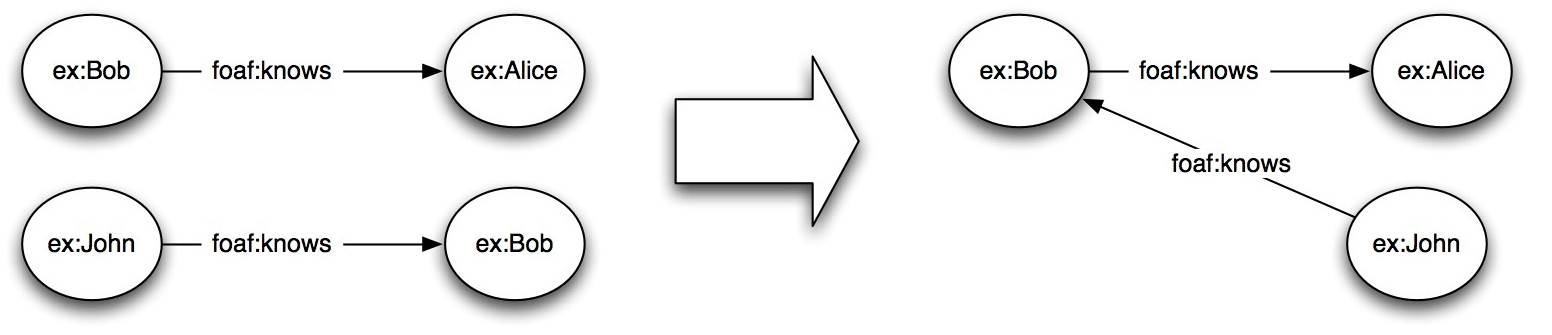
\includegraphics[width=.9\textwidth]
    {./images/triples1-crop}
\end{figure}

Questo insieme di triple RDF (o grafo) può essere espresso, allo scopo di essere scambiato tra applicazioni e pubblicato sul web, in vari formati di serializzazione.

Ad esempio in RDF/XML:
\lstset{ basicstyle=\LSTfont, columns=fullflexible, xleftmargin=5mm, framexleftmargin=5mm, numbers=left, stepnumber=1, breaklines=true, breakatwhitespace=false, numberstyle=\footnotesize, numbersep=5pt, tabsize=2, frame=lines, captionpos=b}
\begin{lstlisting}
<?xml version="1.0"?>
<rdf:RDF
    xmlns:ex="http://example.org/"
    xmlns:foaf="http://xmlns.com/foaf/0.1//"
    xmlns:rdf="http://www.w3.org/1999/02/22-rdf-syntax-ns#">
    <rdf:Description rdf:about="http://example.org/John">
        <foaf:knows>
            <rdf:Description rdf:about="http://example.org/Bob">
                <foaf:knows rdf:resource="http://example.org/Alice" />
            </rdf:Description>
        </foaf:knows>
    </rdf:Description>
</rdf:RDF>
\end{lstlisting}
La caratteristica più importante di tale modello, che si sposa con la visione Linked Data, è usare Uniform Resource Identifier (URI).


=======
Il nostro progetto consiste nella realizzazione di un content-based recommender system che raccomanda film che utilizza i dati provenienti dalla Linked Open Data Cloud per hsdfbjsdhvfhfbsdjfhbsdufh
>>>>>>> 1fd4b5df4f925cfacb4e9dc25651d223388c19b3

	\section{Lavori correlati}
\label{relatedworks}

\citet{mirizzilinked}, affrontando lo stesso problema, hanno utilizzato un VSM puro trasformando il grafo RDF di partenza in un tensore 3-dimensionale di adiacenza.


\citet{passant2010measuring}, invece, in un contesto differente dal nostro (artisti musicali
per poterle confrontare con le nostre

\lipsum

	\section{Progetto}
\label{project}
Il progetto è composto da 5 sezioni:
\begin{itemize}
\item\emph{graph}
\item\emph{distance}
\item\emph{movielens\_exp}
\item\emph{profile}
\item\emph{recommendation}
\end{itemize}
\subsection{graph}
Nella parte iniziale del progetto verranno eseguiti dei metodi presenti nella classi situate all'interno del package \emph{graph}, i cui scopi saranno quelli di: 
\begin{itemize}
\item Salvare all'interno di un grafo i film presenti nel db di movielens;
\item Partendo dal grafo creato in precedenza, viene creato un nuovo grafo in cui ogni vertice rappresenta un film, mentre ogni arco...
\end{itemize}
\subsection{distance}
\subsection{movielens\_exp}
\subsection{profile}
\subsection{recommendation}


Il compito principale di questo modulo consiste inizialmente nella creazione dell'oggetto graph, il cui scopo è quello di contenere in un multigrafo sparso non direzionato le varie risorse estratte dal mapping dei film contenuti nel db di movielens con dbPedia


	\section{Measures}
\label{measures}

	\section{Sperimentazione}
\label{experiment}

Il protocollo sperimentale utilizzato nel progetto, prevede i seguenti passi:
\begin{enumerate}
\item Split del set di ogni utente secondo la proporzione 70/30 (il 70\% del set verrà utilizzato come Training Set, il restante 30\% come Test Set);
\item Per ogni utente:
    \begin{enumerate}
        \item Si creano i due profili utente (pesato e non pesato) utilizzando solo i dati presenti nel suo Training set;
        \item Si creano le liste di raccomandazioni, contenente la totalità dei film, ordinate per importanza, secondo le diverse tipologie di distanza definite nel capitolo \ref{measures};
    \end{enumerate}
\item Calcolo delle due metriche definite nel paragrafo \ref{metriche}
\end{enumerate}

\subsection{Metriche}
\label{metriche}
Al fine di valutare la bontà del sistema creato abbiamo calcolato due tipologie di metriche:
\begin{itemize}
\item Precision
\item MRR
\end{itemize}
Per entrambe le tipologie sono stati presi in esame due punti di vista differenti (\emph{macroscopico} e \emph{microscopico}) ed inoltre, per ogni punto di vista, si è lavorato su due versioni differenti dello stesso dataset (\emph{epurato} e \emph{non epurato}). Questo è stato necessario al fine di migliorare le metriche relative alle raccomandazioni in quanto, nella valutazione, si vanno a considerare solo ed esclusivamente film presenti nel test set (\emph{epurato}) e non nell'intera totalità dei film presenti, di cui nella maggior parte dei casi (film non presenti nel test set) non conosciamo l'opinione dell'utente su quel particolare film (\emph{non epurato}).

\subsubsection{Precision}
In un processo di classificazione statistica, la \emph{precisione} per una classe è il numero di \emph{true positive} (il numero di oggetti etichettati correttamente come appartenenti alla classe) diviso il numero totale di elementi etichettati come appartenenti alla classe (la somma di \emph{true positive} e \emph{false positive}, che sono oggetti etichettati erroneamente come appartenenti alla classe).
Inoltre i termini true positive, true negative, false positive e false negative sono usati per confrontare la classificazione di un oggetto (l’etichetta di classe assegnata all’oggetto da un classificatore) con la corretta classificazione desiderata (la classe a cui in realtà appartiene l’oggetto).
\begin{equation*}
Precision =\frac{TP}{TP+FP}
\end{equation*}

\paragraph{MicroPrecision}
Nel calcolo della microprecisione, è necessario prendere in considerazione i singoli valori di true positive e di false positive di ogni singolo utente come descritto nella formula:
\begin{equation*}
MicroPrecision =\frac{\sum\limits_{u\in U}^{}TP_u}{\sum\limits_{u\in U}^{}TP_u+\sum\limits_{u\in U}^{}FP_u}
\end{equation*}

\paragraph{MacroPrecision}
Per quanto riguarda invece il calcolo della macroprecisione, si va a prendere in considerazione il valor medio delle singole precisioni definite a livello di utente. Formalmente può essere descritto secondo la formula:
\begin{equation*}
MacroPrecision =\frac{1}{|U|}\sum\limits_{u\in U}{Precision_u}
\end{equation*}

\subsubsection{MRR}
Il Mean Reciprocal Rank (MRR) è un indice statistico per valutare un processo che produce una lista di possibili risposte ad una interrogazione (query), ordinate per probabilità di correttezza.
\begin{equation*}
MRR = \frac{1}{|Q|}\sum_{i=1}^{Q}{\frac{1}{Rank_i}}
\end{equation*}

\paragraph{MicroMRR}
Nel calcolo della microMRR, è necessario prendere in considerazione i singoli ranking delle raccomandazioni fatte ad ogni utente come descritto nella formula:
\begin{equation*}
MicroMRR =\frac{\sum\limits_{i=1}^{|R|}{\frac{relevant(r_i)}{i}}}{\sum\limits_{i=1}^{|R|}{\frac{1}{i}}} \qquad relevant(r_i)=\begin{cases} 1 & \mbox{se }r_i\mbox{ è rilevante} \\ 0 & \mbox{altrimenti}
\end{cases}
\end{equation*}
\paragraph{MacroMRR}
Per quanto riguarda invece il calcolo della macroMRR, si va a prendere in considerazione il valor medio dei singoli MRR definiti a livello di utente. Formalmente può essere descritto secondo la formula:
\begin{equation*}
MacroMRR =\frac{1}{|U|}\sum_{u\in U}{MRR_u}
\end{equation*}


	\section{Risultati}
Durante la fase sperimentale sono state testate diversi tipi di configurazioni, assegnando dei valori alle varie proprietà.\footnote{Il valore è compreso nell'intervallo $[0,1]$}; 
Al fine di decidere quali valori possano essere attribuiti alle varie proprietà, sono stati effettuati dei test atti a verificare la qualità e l'importanza che ogni proprietà possa assumere all'atto della raccomandazione. Per fare ciò, sono state create diverse configurazioni nelle quali viene settata solo una proprietà assegnandole il valor massimo plausibile (pari a 1) e annullando le altre proprietà settandole a 0.

\subsection{Configurazione 1}
Nella prima configurazione verrà presa in considerazione solo la proprietà relativa al \emph{subject}; di seguito i risultati della sperimentazione:

\setlength{\tabcolsep}{12pt}
% Table generated by Excel2LaTeX from sheet 'soloSubject'
\begin{table}[H]
	\advance\leftskip-2.5cm
	\resizebox{.9\paperwidth}{!}{%
		\begin{tabular}{ c l r c c c c }
			\toprule
			{\bf $K$} & {\bf $DISTANCE$} & {\bf $PROFILE$} & {\bf $\mu\;\pi$} & {\bf $\mu\;\pi\;$Ts} & {\bf $\mu\;MRR$} & {\bf $\mu\;MRR\;$Ts} \\
			\midrule
				5 &  PASSANT\_D & WEIGHTED & 0,1135399673735730 & 0,6528548123980420 & 0,0665168745759595 & 0,6367328891874240 \\
				
				5 & PASSANT\_D\_W &   WEIGHTED & 0,1063621533442090 & 0,6557911908646000 & 0,0670031759353393 & 0,6344464453125140 \\
				
				5 & PASSANT\_D\_W & NOT\_WEIGHTED & 0,1063621533442090 & 0,6433931484502450 & 0,0681037153634226 & 0,6224393762928970 \\
				
				5 &  PASSANT\_D & NOT\_WEIGHTED & 0,1060358890701470 & 0,6505709624796080 & 0,0674118959128336 & 0,6302953003946530 \\
				
				10 &  PASSANT\_D &   WEIGHTED & 0,0915171288743883 & 0,6206052125240510 & 0,0665168745759595 & 0,6367328891874240 \\
				
				10 & PASSANT\_D\_W & NOT\_WEIGHTED & 0,0911908646003263 & 0,6139583697743570 & 0,0681037153634226 & 0,6224393762928970 \\
				
				10 &  PASSANT\_D & NOT\_WEIGHTED & 0,0898858075040783 & 0,6153577050900820 & 0,0674118959128336 & 0,6302953003946530 \\
				
				10 & PASSANT\_D\_W &   WEIGHTED & 0,0874388254486134 & 0,6218296309253110 & 0,0670031759353393 & 0,6344464453125140 \\
				
				20 &  PASSANT\_D & NOT\_WEIGHTED & 0,0759380097879282 & 0,5850461059882230 & 0,0674118959128336 & 0,6302953003946530 \\
				
				20 & PASSANT\_D\_W & NOT\_WEIGHTED & 0,0744698205546493 & 0,5860459948894570 & 0,0681037153634226 & 0,6224393762928970 \\
				
				20 &  PASSANT\_D &   WEIGHTED & 0,0734910277324633 & 0,5922675258304630 & 0,0665168745759595 & 0,6367328891874240 \\
				
				5 & PASSANT\_C\_W & NOT\_WEIGHTED & 0,0730831973898858 & 0,6306688417618270 & 0,0510441264005910 & 0,6176760233227210 \\
				
				5 & PASSANT\_C\_W &   WEIGHTED & 0,0727569331158238 & 0,6336052202283850 & 0,0504634117165412 & 0,6205882372538300 \\
				
				20 & PASSANT\_D\_W &   WEIGHTED & 0,0721859706362153 & 0,5917120319964450 & 0,0670031759353393 & 0,6344464453125140 \\
				
				5 &  PASSANT\_C & NOT\_WEIGHTED & 0,0681892332789560 & 0,6280587275693310 & 0,0469357759595009 & 0,6192186144970820 \\
				
				5 &  PASSANT\_C &   WEIGHTED & 0,0672104404567700 & 0,6270799347471450 & 0,0470343539139832 & 0,6241689885683380 \\
				
				50 &  PASSANT\_D & NOT\_WEIGHTED & 0,0586949429037520 & 0,5691879585125220 & 0,0674118959128336 & 0,6302953003946530 \\
				
				50 & PASSANT\_D\_W &   WEIGHTED & 0,0580097879282219 & 0,5686820136605110 & 0,0670031759353393 & 0,6344464453125140 \\
				
				10 & PASSANT\_C\_W & NOT\_WEIGHTED & 0,0572593800978793 & 0,6073115270246630 & 0,0510441264005910 & 0,6176760233227210 \\
				
				50 & PASSANT\_D\_W & NOT\_WEIGHTED & 0,0571615008156607 & 0,5685976895185090 & 0,0681037153634226 & 0,6224393762928970 \\
				
				50 &  PASSANT\_D &   WEIGHTED & 0,0569004893964111 & 0,5687663378025130 & 0,0665168745759595 & 0,6367328891874240 \\
				
				10 &  PASSANT\_C & NOT\_WEIGHTED & 0,0567699836867863 & 0,6087108623403880 & 0,0469357759595009 & 0,6192186144970820 \\
				
				10 & PASSANT\_C\_W &   WEIGHTED & 0,0562805872756933 & 0,6076613608535950 & 0,0504634117165412 & 0,6205882372538300 \\
				
				10 &  PASSANT\_C &   WEIGHTED & 0,0562805872756933 & 0,6076613608535950 & 0,0470343539139832 & 0,6241689885683380 \\
				
				20 & PASSANT\_C\_W &   WEIGHTED & 0,0506525285481240 & 0,5824908343517390 & 0,0504634117165412 & 0,6205882372538300 \\
				
				20 & PASSANT\_C\_W & NOT\_WEIGHTED & 0,0496737357259380 & 0,5802688590156650 & 0,0510441264005910 & 0,6176760233227210 \\
				
				100 &  PASSANT\_D & NOT\_WEIGHTED & 0,0476672104404568 & 0,5662331207025100 & 0,0674118959128336 & 0,6302953003946530 \\
				
				100 & PASSANT\_D\_W & NOT\_WEIGHTED & 0,0476182707993475 & 0,5662331207025100 & 0,0681037153634226 & 0,6224393762928970 \\
				
				100 & PASSANT\_D\_W &   WEIGHTED & 0,0468026101141925 & 0,5662331207025100 & 0,0670031759353393 & 0,6344464453125140 \\
				
				100 &  PASSANT\_D &   WEIGHTED & 0,0466394779771615 & 0,5662331207025100 & 0,0665168745759595 & 0,6367328891874240 \\
				
				20 &  PASSANT\_C &   WEIGHTED & 0,0459216965742251 & 0,5832685257193640 & 0,0470343539139832 & 0,6241689885683380 \\
				
				20 &  PASSANT\_C & NOT\_WEIGHTED & 0,0457585644371941 & 0,5813798466837020 & 0,0469357759595009 & 0,6192186144970820 \\
				
				50 & PASSANT\_C\_W & NOT\_WEIGHTED & 0,0429037520391517 & 0,5688506619445150 & 0,0510441264005910 & 0,6176760233227210 \\
				
				50 & PASSANT\_C\_W &   WEIGHTED & 0,0428711256117455 & 0,5686820136605110 & 0,0504634117165412 & 0,6205882372538300 \\
				
				50 &  PASSANT\_C & NOT\_WEIGHTED & 0,0410440456769984 & 0,5687663378025130 & 0,0469357759595009 & 0,6192186144970820 \\
				
				50 &  PASSANT\_C &   WEIGHTED & 0,0408156606851550 & 0,5687663378025130 & 0,0470343539139832 & 0,6241689885683380 \\
				
				100 & PASSANT\_C\_W & NOT\_WEIGHTED & 0,0382544861337684 & 0,5662331207025100 & 0,0510441264005910 & 0,6176760233227210 \\
				
				100 & PASSANT\_C\_W &   WEIGHTED & 0,0374551386623165 & 0,5662331207025100 & 0,0504634117165412 & 0,6205882372538300 \\
				
				100 &  PASSANT\_C & NOT\_WEIGHTED & 0,0364926590538336 & 0,5662331207025100 & 0,0469357759595009 & 0,6192186144970820 \\
				
				100 &  PASSANT\_C &   WEIGHTED & 0,0363295269168026 & 0,5662331207025100 & 0,0470343539139832 & 0,6241689885683380 \\
			\bottomrule
		\end{tabular}
}
\caption{\emph{Risultati configurazione 1 - solo subject}}
\end{table}

\setlength{\tabcolsep}{12pt}
% Table generated by Excel2LaTeX from sheet 'soloSubject'
\begin{table}[H]
		\advance\leftskip-2.5cm
		\resizebox{.9\paperwidth}{!}{%
			\begin{tabular}{ c l r c c c c }
				\toprule
				{\bf $K$} & {\bf $DISTANCE$} & {\bf $PROFILE$} & {\bf $M\;\pi$} & {\bf $M\;\pi\;$Ts} & {\bf $M\;MRR$} & {\bf $M\;MRR\;$Ts} \\
				\midrule
	5 &  PASSANT\_D &   WEIGHTED & 0,1135399673735730 & 0,6528548123980440 & 0,0668442309630926 & 0,6414757672167860 \\
	
	5 & PASSANT\_D\_W &   WEIGHTED & 0,1063621533442090 & 0,6557911908646020 & 0,0673057937032880 & 0,6387603251875660 \\
	
	5 & PASSANT\_D\_W & NOT\_WEIGHTED & 0,1063621533442090 & 0,6433931484502460 & 0,0682954594049652 & 0,6278338027357970 \\
	
	5 &  PASSANT\_D & NOT\_WEIGHTED & 0,1060358890701470 & 0,6505709624796110 & 0,0675978796074208 & 0,6358315445908260 \\
	
	10 &  PASSANT\_D &   WEIGHTED & 0,0915171288743886 & 0,6229051762086020 & 0,0668442309630926 & 0,6414757672167860 \\
	
	10 & PASSANT\_D\_W & NOT\_WEIGHTED & 0,0911908646003266 & 0,6167061550014240 & 0,0682954594049652 & 0,6278338027357970 \\
	
	10 &  PASSANT\_D & NOT\_WEIGHTED & 0,0898858075040787 & 0,6180112120976730 & 0,0675978796074208 & 0,6358315445908260 \\
	
	10 & PASSANT\_D\_W &   WEIGHTED & 0,0874388254486137 & 0,6240471011678190 & 0,0673057937032880 & 0,6387603251875660 \\
	
	20 &  PASSANT\_D & NOT\_WEIGHTED & 0,0759380097879282 & 0,5967615743754140 & 0,0675978796074208 & 0,6358315445908260 \\
	
	20 & PASSANT\_D\_W & NOT\_WEIGHTED & 0,0744698205546492 & 0,5974956689920530 & 0,0682954594049652 & 0,6278338027357970 \\
	
	20 &  PASSANT\_D &   WEIGHTED & 0,0734910277324632 & 0,6020633688289210 & 0,0668442309630926 & 0,6414757672167860 \\
	
	5 & PASSANT\_C\_W & NOT\_WEIGHTED & 0,0730831973898859 & 0,6306688417618280 & 0,0512218251867321 & 0,6246363752298640 \\
	
	5 & PASSANT\_C\_W &   WEIGHTED & 0,0727569331158239 & 0,6336052202283870 & 0,0507352353727599 & 0,6270519487403240 \\
	
	20 & PASSANT\_D\_W &   WEIGHTED & 0,0721859706362153 & 0,6016555384863430 & 0,0673057937032880 & 0,6387603251875660 \\
	
	5 &  PASSANT\_C & NOT\_WEIGHTED & 0,0681892332789560 & 0,6280587275693330 & 0,0470782803480684 & 0,6262790723706200 \\
	
	5 &  PASSANT\_C &   WEIGHTED & 0,0672104404567700 & 0,6270799347471470 & 0,0472549045028841 & 0,6305515857308470 \\
	
	50 &  PASSANT\_D & NOT\_WEIGHTED & 0,0586949429037518 & 0,5912138989521130 & 0,0675978796074208 & 0,6358315445908260 \\
	
	50 & PASSANT\_D\_W &   WEIGHTED & 0,0580097879282217 & 0,5910181403876760 & 0,0673057937032880 & 0,6387603251875660 \\
	
	10 & PASSANT\_C\_W & NOT\_WEIGHTED & 0,0572593800978794 & 0,6105071337942460 & 0,0512218251867321 & 0,6246363752298640 \\
	
	50 & PASSANT\_D\_W & NOT\_WEIGHTED & 0,0571615008156605 & 0,5909855139602700 & 0,0682954594049652 & 0,6278338027357970 \\
	
	50 &  PASSANT\_D &   WEIGHTED & 0,0569004893964109 & 0,5910507668150820 & 0,0668442309630926 & 0,6414757672167860 \\
	
	10 &  PASSANT\_C & NOT\_WEIGHTED & 0,0567699836867864 & 0,6118121908904940 & 0,0470782803480684 & 0,6262790723706200 \\
	
	10 & PASSANT\_C\_W &   WEIGHTED & 0,0562805872756935 & 0,6108333980683080 & 0,0507352353727599 & 0,6270519487403240 \\
	
	10 &  PASSANT\_C &   WEIGHTED & 0,0562805872756935 & 0,6108333980683080 & 0,0472549045028841 & 0,6305515857308470 \\
	
	20 & PASSANT\_C\_W &   WEIGHTED & 0,0506525285481242 & 0,5948855547995570 & 0,0507352353727599 & 0,6270519487403240 \\
	
	20 & PASSANT\_C\_W & NOT\_WEIGHTED & 0,0496737357259382 & 0,5932542334292470 & 0,0512218251867321 & 0,6246363752298640 \\
	
	100 &  PASSANT\_D & NOT\_WEIGHTED & 0,0476672104404568 & 0,5907987598795780 & 0,0675978796074208 & 0,6358315445908260 \\
	
	100 & PASSANT\_D\_W & NOT\_WEIGHTED & 0,0476182707993475 & 0,5907987598795780 & 0,0682954594049652 & 0,6278338027357970 \\
	
	100 & PASSANT\_D\_W &   WEIGHTED & 0,0468026101141925 & 0,5907987598795780 & 0,0673057937032880 & 0,6387603251875660 \\
	
	100 &  PASSANT\_D &   WEIGHTED & 0,0466394779771615 & 0,5907987598795780 & 0,0668442309630926 & 0,6414757672167860 \\
	
	20 &  PASSANT\_C &   WEIGHTED & 0,0459216965742253 & 0,5954565172791660 & 0,0472549045028841 & 0,6305515857308470 \\
	
	20 &  PASSANT\_C & NOT\_WEIGHTED & 0,0457585644371943 & 0,5940698941144020 & 0,0470782803480684 & 0,6262790723706200 \\
	
	50 & PASSANT\_C\_W & NOT\_WEIGHTED & 0,0429037520391514 & 0,5910833932424880 & 0,0512218251867321 & 0,6246363752298640 \\
	
	50 & PASSANT\_C\_W &   WEIGHTED & 0,0428711256117452 & 0,5910181403876760 & 0,0507352353727599 & 0,6270519487403240 \\
	
	50 &  PASSANT\_C & NOT\_WEIGHTED & 0,0410440456769981 & 0,5910507668150820 & 0,0470782803480684 & 0,6262790723706200 \\
	
	50 &  PASSANT\_C &   WEIGHTED & 0,0408156606851547 & 0,5910507668150820 & 0,0472549045028841 & 0,6305515857308470 \\
	
	100 & PASSANT\_C\_W & NOT\_WEIGHTED & 0,0382544861337684 & 0,5907987598795780 & 0,0512218251867321 & 0,6246363752298640 \\
	
	100 & PASSANT\_C\_W &   WEIGHTED & 0,0374551386623165 & 0,5907987598795780 & 0,0507352353727599 & 0,6270519487403240 \\
	
	100 &  PASSANT\_C & NOT\_WEIGHTED & 0,0364926590538336 & 0,5907987598795780 & 0,0470782803480684 & 0,6262790723706200 \\
	
	100 &  PASSANT\_C &   WEIGHTED & 0,0363295269168026 & 0,5907987598795780 & 0,0472549045028841 & 0,6305515857308470 \\
	\bottomrule
\end{tabular}  
}
\caption{\emph{Risultati configurazione 1 - solo subject}}
\end{table} 

\subsection{Configurazione 2}
Nella seconda configurazione verrà presa in considerazione solo la proprietà relativa al \emph{director}; di seguito i risultati della sperimentazione:

\setlength{\tabcolsep}{12pt}
% Table generated by Excel2LaTeX from sheet 'soloDirector'
\begin{table}[H]
	\advance\leftskip-2.5cm
	\resizebox{.9\paperwidth}{!}{%
		\begin{tabular}{ c l r c c c c }
			\toprule
			{\bf $K$} & {\bf $DISTANCE$} & {\bf $PROFILE$} & {\bf $\mu\;\pi$} & {\bf $\mu\;\pi\;$Ts} & {\bf $\mu\;MRR$} & {\bf $\mu\;MRR\;$Ts} \\
			\midrule
				5 &  PASSANT\_D &   WEIGHTED & 0,1135399673735730 & 0,6528548123980420 & 0,0665168745759595 & 0,6367328891874240 \\
				
				5 & PASSANT\_D\_W &   WEIGHTED & 0,1112561174551390 & 0,6646003262642740 & 0,0726799071544549 & 0,6495391427644200 \\
				
				5 & PASSANT\_D\_W & NOT\_WEIGHTED & 0,1092985318107670 & 0,6636215334420880 & 0,0687312959140887 & 0,6476203531668750 \\
				
				5 &  PASSANT\_D & NOT\_WEIGHTED & 0,1060358890701470 & 0,6505709624796080 & 0,0674118959128336 & 0,6302953003946530 \\
				
				5 & PASSANT\_C\_W &   WEIGHTED & 0,0972267536704731 & 0,6603588907014680 & 0,0693418945114162 & 0,6461280924797000 \\
				
				10 & PASSANT\_D\_W & NOT\_WEIGHTED & 0,0955954323001632 & 0,6295259751617980 & 0,0687312959140887 & 0,6476203531668750 \\
				
				10 & PASSANT\_D\_W &   WEIGHTED & 0,0933115823817292 & 0,6324995627077140 & 0,0726799071544549 & 0,6495391427644200 \\
				
				10 &  PASSANT\_D &   WEIGHTED & 0,0915171288743883 & 0,6206052125240510 & 0,0665168745759595 & 0,6367328891874240 \\
				
				10 &  PASSANT\_D & NOT\_WEIGHTED & 0,0898858075040783 & 0,6153577050900820 & 0,0674118959128336 & 0,6302953003946530 \\
				
				10 & PASSANT\_C\_W &   WEIGHTED & 0,0895595432300163 & 0,6324995627077140 & 0,0693418945114162 & 0,6461280924797000 \\
				
				5 & PASSANT\_C\_W & NOT\_WEIGHTED & 0,0864600326264274 & 0,6587275693311580 & 0,0633985884037322 & 0,6428454795256440 \\
				
				10 & PASSANT\_C\_W & NOT\_WEIGHTED & 0,0820554649265905 & 0,6298758089907290 & 0,0633985884037322 & 0,6428454795256440 \\
				
				20 & PASSANT\_D\_W &   WEIGHTED & 0,0765905383360522 & 0,6012665259415620 & 0,0726799071544549 & 0,6495391427644200 \\
				
				20 & PASSANT\_C\_W &   WEIGHTED & 0,0763458401305057 & 0,6012665259415620 & 0,0693418945114162 & 0,6461280924797000 \\
				
				20 &  PASSANT\_D & NOT\_WEIGHTED & 0,0759380097879282 & 0,5850461059882230 & 0,0674118959128336 & 0,6302953003946530 \\
				
				20 &  PASSANT\_D &   WEIGHTED & 0,0734910277324633 & 0,5922675258304630 & 0,0665168745759595 & 0,6367328891874240 \\
				
				20 & PASSANT\_C\_W & NOT\_WEIGHTED & 0,0730016313213703 & 0,6001555382735250 & 0,0633985884037322 & 0,6428454795256440 \\
				
				20 & PASSANT\_D\_W & NOT\_WEIGHTED & 0,0720228384991843 & 0,6001555382735250 & 0,0687312959140887 & 0,6476203531668750 \\
				
				5 &  PASSANT\_C & NOT\_WEIGHTED & 0,0681892332789560 & 0,6280587275693310 & 0,0469357759595009 & 0,6192186144970820 \\
				
				5 &  PASSANT\_C &   WEIGHTED & 0,0672104404567700 & 0,6270799347471450 & 0,0470343539139832 & 0,6241689885683380 \\
				
				50 & PASSANT\_D\_W &   WEIGHTED & 0,0624143556280587 & 0,5703684965005480 & 0,0726799071544549 & 0,6495391427644200 \\
				
				50 & PASSANT\_C\_W &   WEIGHTED & 0,0622185970636215 & 0,5703684965005480 & 0,0693418945114162 & 0,6461280924797000 \\
				
				100 & PASSANT\_D\_W &   WEIGHTED & 0,0588254486133768 & 0,5662331207025100 & 0,0726799071544549 & 0,6495391427644200 \\
				
				100 & PASSANT\_C\_W &   WEIGHTED & 0,0587765089722675 & 0,5662331207025100 & 0,0693418945114162 & 0,6461280924797000 \\
				
				50 &  PASSANT\_D & NOT\_WEIGHTED & 0,0586949429037520 & 0,5691879585125220 & 0,0674118959128336 & 0,6302953003946530 \\
				
				50 & PASSANT\_D\_W & NOT\_WEIGHTED & 0,0576835236541599 & 0,5704528206425500 & 0,0687312959140887 & 0,6476203531668750 \\
				
				50 & PASSANT\_C\_W & NOT\_WEIGHTED & 0,0574551386623165 & 0,5704528206425500 & 0,0633985884037322 & 0,6428454795256440 \\
				
				100 & PASSANT\_D\_W & NOT\_WEIGHTED & 0,0569168026101142 & 0,5662331207025100 & 0,0687312959140887 & 0,6476203531668750 \\
				
				50 &  PASSANT\_D &   WEIGHTED & 0,0569004893964111 & 0,5687663378025130 & 0,0665168745759595 & 0,6367328891874240 \\
				
				100 & PASSANT\_C\_W & NOT\_WEIGHTED & 0,0568189233278956 & 0,5662331207025100 & 0,0633985884037322 & 0,6428454795256440 \\
				
				10 &  PASSANT\_C & NOT\_WEIGHTED & 0,0567699836867863 & 0,6087108623403880 & 0,0469357759595009 & 0,6192186144970820 \\
				
				10 &  PASSANT\_C &   WEIGHTED & 0,0562805872756933 & 0,6076613608535950 & 0,0470343539139832 & 0,6241689885683380 \\
				
				100 &  PASSANT\_D & NOT\_WEIGHTED & 0,0476672104404568 & 0,5662331207025100 & 0,0674118959128336 & 0,6302953003946530 \\
				
				100 &  PASSANT\_D &   WEIGHTED & 0,0466394779771615 & 0,5662331207025100 & 0,0665168745759595 & 0,6367328891874240 \\
				
				20 &  PASSANT\_C &   WEIGHTED & 0,0459216965742251 & 0,5832685257193640 & 0,0470343539139832 & 0,6241689885683380 \\
				
				20 &  PASSANT\_C & NOT\_WEIGHTED & 0,0457585644371941 & 0,5813798466837020 & 0,0469357759595009 & 0,6192186144970820 \\
				
				50 &  PASSANT\_C & NOT\_WEIGHTED & 0,0410440456769984 & 0,5687663378025130 & 0,0469357759595009 & 0,6192186144970820 \\
				
				50 &  PASSANT\_C &   WEIGHTED & 0,0408156606851550 & 0,5687663378025130 & 0,0470343539139832 & 0,6241689885683380 \\
				
				100 &  PASSANT\_C & NOT\_WEIGHTED & 0,0364926590538336 & 0,5662331207025100 & 0,0469357759595009 & 0,6192186144970820 \\
				
				100 &  PASSANT\_C &   WEIGHTED & 0,0363295269168026 & 0,5662331207025100 & 0,0470343539139832 & 0,6241689885683380 \\			
			\bottomrule
		\end{tabular}  
	}
	\caption{\emph{Risultati configurazione 2 - solo Director}}
\end{table}

\setlength{\tabcolsep}{12pt}
% Table generated by Excel2LaTeX from sheet 'soloDirector'
\begin{table}[H]
	\advance\leftskip-2.5cm
	\resizebox{.9\paperwidth}{!}{%
		\begin{tabular}{ c l r c c c c }
			\toprule
			{\bf $K$} & {\bf $DISTANCE$} & {\bf $PROFILE$} & {\bf $M\;\pi$} & {\bf $M\;\pi\;$Ts} & {\bf $M\;MRR$} & {\bf $M\;MRR\;$Ts} \\
			\midrule
				5 &  PASSANT\_D &   WEIGHTED & 0,1135399673735730 & 0,6528548123980440 & 0,0668442309630926 & 0,6414757672167860 \\
				
				5 & PASSANT\_D\_W &   WEIGHTED & 0,1112561174551390 & 0,6646003262642760 & 0,0732004886413820 & 0,6525942110169710 \\
				
				5 & PASSANT\_D\_W & NOT\_WEIGHTED & 0,1092985318107670 & 0,6636215334420900 & 0,0690576171961171 & 0,6508044323270640 \\
				
				5 &  PASSANT\_D & NOT\_WEIGHTED & 0,1060358890701470 & 0,6505709624796110 & 0,0675978796074208 & 0,6358315445908260 \\
				
				5 & PASSANT\_C\_W &   WEIGHTED & 0,0972267536704733 & 0,6603588907014700 & 0,0698514313285939 & 0,6496409646246790 \\
				
				10 & PASSANT\_D\_W & NOT\_WEIGHTED & 0,0955954323001635 & 0,6312249151971830 & 0,0690576171961171 & 0,6508044323270640 \\
				
				10 & PASSANT\_D\_W &   WEIGHTED & 0,0933115823817296 & 0,6339981615267100 & 0,0732004886413820 & 0,6525942110169710 \\
				
				10 &  PASSANT\_D &   WEIGHTED & 0,0915171288743886 & 0,6229051762086020 & 0,0668442309630926 & 0,6414757672167860 \\
				
				10 &  PASSANT\_D & NOT\_WEIGHTED & 0,0898858075040787 & 0,6180112120976730 & 0,0675978796074208 & 0,6358315445908260 \\
				
				10 & PASSANT\_C\_W &   WEIGHTED & 0,0895595432300167 & 0,6339981615267090 & 0,0698514313285939 & 0,6496409646246790 \\
				
				5 & PASSANT\_C\_W & NOT\_WEIGHTED & 0,0864600326264276 & 0,6587275693311600 & 0,0637039131554447 & 0,6470860235878480 \\
				
				10 & PASSANT\_C\_W & NOT\_WEIGHTED & 0,0820554649265909 & 0,6315511794712450 & 0,0637039131554447 & 0,6470860235878480 \\
				
				20 & PASSANT\_D\_W &   WEIGHTED & 0,0765905383360521 & 0,6086702203786760 & 0,0732004886413820 & 0,6525942110169710 \\
				
				20 & PASSANT\_C\_W &   WEIGHTED & 0,0763458401305057 & 0,6086702203786760 & 0,0698514313285939 & 0,6496409646246790 \\
				
				20 &  PASSANT\_D & NOT\_WEIGHTED & 0,0759380097879282 & 0,5967615743754140 & 0,0675978796074208 & 0,6358315445908260 \\
				
				20 &  PASSANT\_D &   WEIGHTED & 0,0734910277324632 & 0,6020633688289210 & 0,0668442309630926 & 0,6414757672167860 \\
				
				20 & PASSANT\_C\_W & NOT\_WEIGHTED & 0,0730016313213703 & 0,6078545596935210 & 0,0637039131554447 & 0,6470860235878480 \\
				
				20 & PASSANT\_D\_W & NOT\_WEIGHTED & 0,0720228384991843 & 0,6078545596935210 & 0,0690576171961171 & 0,6508044323270640 \\
				
				5 &  PASSANT\_C & NOT\_WEIGHTED & 0,0681892332789560 & 0,6280587275693330 & 0,0470782803480684 & 0,6262790723706200 \\
				
				5 &  PASSANT\_C &   WEIGHTED & 0,0672104404567700 & 0,6270799347471470 & 0,0472549045028841 & 0,6305515857308470 \\
				
				50 & PASSANT\_D\_W &   WEIGHTED & 0,0624143556280586 & 0,5916706689358000 & 0,0732004886413820 & 0,6525942110169710 \\
				
				50 & PASSANT\_C\_W &   WEIGHTED & 0,0622185970636214 & 0,5916706689358000 & 0,0698514313285939 & 0,6496409646246790 \\
				
				100 & PASSANT\_D\_W &   WEIGHTED & 0,0588254486133769 & 0,5907987598795780 & 0,0732004886413820 & 0,6525942110169710 \\
				
				100 & PASSANT\_C\_W &   WEIGHTED & 0,0587765089722676 & 0,5907987598795780 & 0,0698514313285939 & 0,6496409646246790 \\
				
				50 &  PASSANT\_D & NOT\_WEIGHTED & 0,0586949429037518 & 0,5912138989521130 & 0,0675978796074208 & 0,6358315445908260 \\
				
				50 & PASSANT\_D\_W & NOT\_WEIGHTED & 0,0576835236541597 & 0,5917032953632060 & 0,0690576171961171 & 0,6508044323270640 \\
				
				50 & PASSANT\_C\_W & NOT\_WEIGHTED & 0,0574551386623163 & 0,5917032953632060 & 0,0637039131554447 & 0,6470860235878480 \\
				
				100 & PASSANT\_D\_W & NOT\_WEIGHTED & 0,0569168026101142 & 0,5907987598795780 & 0,0690576171961171 & 0,6508044323270640 \\
				
				50 &  PASSANT\_D &   WEIGHTED & 0,0569004893964109 & 0,5910507668150820 & 0,0668442309630926 & 0,6414757672167860 \\
				
				100 & PASSANT\_C\_W & NOT\_WEIGHTED & 0,0568189233278956 & 0,5907987598795780 & 0,0637039131554447 & 0,6470860235878480 \\
				
				10 &  PASSANT\_C & NOT\_WEIGHTED & 0,0567699836867864 & 0,6118121908904940 & 0,0470782803480684 & 0,6262790723706200 \\
				
				10 &  PASSANT\_C &   WEIGHTED & 0,0562805872756935 & 0,6108333980683080 & 0,0472549045028841 & 0,6305515857308470 \\
				
				100 &  PASSANT\_D & NOT\_WEIGHTED & 0,0476672104404568 & 0,5907987598795780 & 0,0675978796074208 & 0,6358315445908260 \\
				
				100 &  PASSANT\_D &   WEIGHTED & 0,0466394779771615 & 0,5907987598795780 & 0,0668442309630926 & 0,6414757672167860 \\
				
				20 &  PASSANT\_C &   WEIGHTED & 0,0459216965742253 & 0,5954565172791660 & 0,0472549045028841 & 0,6305515857308470 \\
				
				20 &  PASSANT\_C & NOT\_WEIGHTED & 0,0457585644371943 & 0,5940698941144020 & 0,0470782803480684 & 0,6262790723706200 \\
				
				50 &  PASSANT\_C & NOT\_WEIGHTED & 0,0410440456769981 & 0,5910507668150820 & 0,0470782803480684 & 0,6262790723706200 \\
				
				50 &  PASSANT\_C &   WEIGHTED & 0,0408156606851547 & 0,5910507668150820 & 0,0472549045028841 & 0,6305515857308470 \\
				
				100 &  PASSANT\_C & NOT\_WEIGHTED & 0,0364926590538336 & 0,5907987598795780 & 0,0470782803480684 & 0,6262790723706200 \\
				
				100 &  PASSANT\_C &   WEIGHTED & 0,0363295269168026 & 0,5907987598795780 & 0,0472549045028841 & 0,6305515857308470 \\
			\bottomrule
		\end{tabular}  
	}
	\caption{\emph{Risultati configurazione 2 - solo Director}}
\end{table} 


\subsection{Configurazione 3}
Nella terza configurazione verrà presa in considerazione solo la proprietà relativa al \emph{producer}; di seguito i risultati della sperimentazione:

\setlength{\tabcolsep}{12pt}
% Table generated by Excel2LaTeX from sheet 'soloProducer'
\begin{table}[H]
	\advance\leftskip-2.5cm
	\resizebox{.9\paperwidth}{!}{%
		\begin{tabular}{ c l r c c c c }
			\toprule
			{\bf $K$} & {\bf $DISTANCE$} & {\bf $PROFILE$} & {\bf $\mu\;\pi$} & {\bf $\mu\;\pi\;$Ts} & {\bf $\mu\;MRR$} & {\bf $\mu\;MRR\;$Ts} \\
			\midrule		
				10 &  PASSANT\_D & NOT\_WEIGHTED & 0,1135399673735730 & 0,6528548123980420 & 0,0665168745759595 & 0,6367328891874240 \\
				
				5 &  PASSANT\_D &   WEIGHTED & 0,1060358890701470 & 0,6505709624796080 & 0,0674118959128336 & 0,6302953003946530 \\
				
				10 &  PASSANT\_C & NOT\_WEIGHTED & 0,0915171288743883 & 0,6206052125240510 & 0,0665168745759595 & 0,6367328891874240 \\
				
				5 &  PASSANT\_D & NOT\_WEIGHTED & 0,0898858075040783 & 0,6153577050900820 & 0,0674118959128336 & 0,6302953003946530 \\
				
				5 &  PASSANT\_C & NOT\_WEIGHTED & 0,0759380097879282 & 0,5850461059882230 & 0,0674118959128336 & 0,6302953003946530 \\
				
				10 &  PASSANT\_C &   WEIGHTED & 0,0734910277324633 & 0,5922675258304630 & 0,0665168745759595 & 0,6367328891874240 \\
				
				50 &  PASSANT\_C & NOT\_WEIGHTED & 0,0681892332789560 & 0,6280587275693310 & 0,0469357759595009 & 0,6192186144970820 \\
				
				50 &  PASSANT\_C &   WEIGHTED & 0,0681892332789560 & 0,6280587275693310 & 0,0469357759595009 & 0,6192186144970820 \\
				
				20 &  PASSANT\_C &   WEIGHTED & 0,0672104404567700 & 0,6270799347471450 & 0,0470343539139832 & 0,6241689885683380 \\
				
				5 & PASSANT\_D\_W &   WEIGHTED & 0,0659053833605220 & 0,6453507340946170 & 0,0492489814586122 & 0,6338333099711730 \\
				
				5 &  PASSANT\_C &   WEIGHTED & 0,0586949429037520 & 0,5691879585125220 & 0,0674118959128336 & 0,6302953003946530 \\
				
				10 & PASSANT\_D\_W &   WEIGHTED & 0,0574225122349103 & 0,6193807941227920 & 0,0492489814586122 & 0,6338333099711730 \\
				
				20 &  PASSANT\_D &   WEIGHTED & 0,0569004893964111 & 0,5687663378025130 & 0,0665168745759595 & 0,6367328891874240 \\
				
				20 &  PASSANT\_C & NOT\_WEIGHTED & 0,0562805872756933 & 0,6076613608535950 & 0,0470343539139832 & 0,6241689885683380 \\
				
				5 & PASSANT\_D\_W & NOT\_WEIGHTED & 0,0557911908646003 & 0,6407830342577490 & 0,0459999049131870 & 0,6290527698935050 \\
				
				100 & PASSANT\_D\_W &   WEIGHTED & 0,0540619902120718 & 0,5662331207025100 & 0,0492489814586122 & 0,6338333099711730 \\
				
				20 & PASSANT\_D\_W &   WEIGHTED & 0,0528548123980424 & 0,5951560937673590 & 0,0492489814586122 & 0,6338333099711730 \\
				
				5 & PASSANT\_C\_W &   WEIGHTED & 0,0505709624796085 & 0,6339314845024470 & 0,0446164357419806 & 0,6209528087891790 \\
				
				100 & PASSANT\_D\_W & NOT\_WEIGHTED & 0,0503752039151713 & 0,5662331207025100 & 0,0459999049131870 & 0,6290527698935050 \\
				
				50 & PASSANT\_D\_W &   WEIGHTED & 0,0496574225122349 & 0,5701155240745430 & 0,0492489814586122 & 0,6338333099711730 \\
				
				20 & PASSANT\_D\_W & NOT\_WEIGHTED & 0,0491027732463295 & 0,5943784023997330 & 0,0459999049131870 & 0,6290527698935050 \\
				
				100 & PASSANT\_C\_W &   WEIGHTED & 0,0487112561174551 & 0,5662331207025100 & 0,0446164357419806 & 0,6209528087891790 \\
				
				10 & PASSANT\_D\_W & NOT\_WEIGHTED & 0,0484502446982055 & 0,6188560433793950 & 0,0459999049131870 & 0,6290527698935050 \\
				
				10 &  PASSANT\_D &   WEIGHTED & 0,0476672104404568 & 0,5662331207025100 & 0,0674118959128336 & 0,6302953003946530 \\
				
				20 &  PASSANT\_D & NOT\_WEIGHTED & 0,0466394779771615 & 0,5662331207025100 & 0,0665168745759595 & 0,6367328891874240 \\
				
				50 & PASSANT\_D\_W & NOT\_WEIGHTED & 0,0465252854812398 & 0,5702841723585460 & 0,0459999049131870 & 0,6290527698935050 \\
				
				50 &  PASSANT\_D & NOT\_WEIGHTED & 0,0459216965742251 & 0,5832685257193640 & 0,0470343539139832 & 0,6241689885683380 \\
				
				100 &  PASSANT\_D & NOT\_WEIGHTED & 0,0457585644371941 & 0,5813798466837020 & 0,0469357759595009 & 0,6192186144970820 \\
				
				100 &  PASSANT\_D &   WEIGHTED & 0,0457585644371941 & 0,5813798466837020 & 0,0469357759595009 & 0,6192186144970820 \\
				
				10 & PASSANT\_C\_W &   WEIGHTED & 0,0453507340946166 & 0,6144831205177540 & 0,0446164357419806 & 0,6209528087891790 \\
				
				100 & PASSANT\_C\_W & NOT\_WEIGHTED & 0,0447308319738989 & 0,5662331207025100 & 0,0420353204004616 & 0,6199350427006180 \\
				
				50 & PASSANT\_C\_W &   WEIGHTED & 0,0445676998368679 & 0,5696095792225310 & 0,0446164357419806 & 0,6209528087891790 \\
				
				20 & PASSANT\_C\_W &   WEIGHTED & 0,0437194127243067 & 0,5921564270636600 & 0,0446164357419806 & 0,6209528087891790 \\
				
				50 & PASSANT\_C\_W & NOT\_WEIGHTED & 0,0422512234910277 & 0,5700311999325410 & 0,0420353204004616 & 0,6199350427006180 \\
				
				5 & PASSANT\_C\_W & NOT\_WEIGHTED & 0,0414355628058728 & 0,6264274061990210 & 0,0420353204004616 & 0,6199350427006180 \\
				
				20 & PASSANT\_C\_W & NOT\_WEIGHTED & 0,0410277324632953 & 0,5898233529607820 & 0,0420353204004616 & 0,6199350427006180 \\
				
				50 &  PASSANT\_D &   WEIGHTED & 0,0408156606851550 & 0,5687663378025130 & 0,0470343539139832 & 0,6241689885683380 \\
				
				10 & PASSANT\_C\_W & NOT\_WEIGHTED & 0,0378466557911909 & 0,6125590344586320 & 0,0420353204004616 & 0,6199350427006180 \\
				
				100 &  PASSANT\_C & NOT\_WEIGHTED & 0,0364926590538336 & 0,5662331207025100 & 0,0469357759595009 & 0,6192186144970820 \\
				
				100 &  PASSANT\_C &   WEIGHTED & 0,0364926590538336 & 0,5662331207025100 & 0,0469357759595009 & 0,6192186144970820 \\
			\bottomrule
		\end{tabular}  
	}
	\caption{\emph{Risultati configurazione 3 - solo Producer}}
\end{table}

\setlength{\tabcolsep}{12pt}
% Table generated by Excel2LaTeX from sheet 'soloProducer'
\begin{table}[H]
	\advance\leftskip-2.5cm
	\resizebox{.9\paperwidth}{!}{%
		\begin{tabular}{ c l r c c c c }
			\toprule
			{\bf $K$} & {\bf $DISTANCE$} & {\bf $PROFILE$} & {\bf $M\;\pi$} & {\bf $M\;\pi\;$Ts} & {\bf $M\;MRR$} & {\bf $M\;MRR\;$Ts} \\
			\midrule
				10 &  PASSANT\_D & NOT\_WEIGHTED & 0,1135399673735730 & 0,6528548123980440 & 0,0668442309630926 & 0,6414757672167860 \\
				
				5 &  PASSANT\_D &   WEIGHTED & 0,1060358890701470 & 0,6505709624796110 & 0,0675978796074208 & 0,6358315445908260 \\
				
				10 &  PASSANT\_C & NOT\_WEIGHTED & 0,0915171288743886 & 0,6229051762086020 & 0,0668442309630926 & 0,6414757672167860 \\
				
				5 &  PASSANT\_D & NOT\_WEIGHTED & 0,0898858075040787 & 0,6180112120976730 & 0,0675978796074208 & 0,6358315445908260 \\
				
				5 &  PASSANT\_C & NOT\_WEIGHTED & 0,0759380097879282 & 0,5967615743754140 & 0,0675978796074208 & 0,6358315445908260 \\
				
				10 &  PASSANT\_C &   WEIGHTED & 0,0734910277324632 & 0,6020633688289210 & 0,0668442309630926 & 0,6414757672167860 \\
				
				50 &  PASSANT\_C & NOT\_WEIGHTED & 0,0681892332789560 & 0,6280587275693330 & 0,0470782803480684 & 0,6262790723706200 \\
				
				50 &  PASSANT\_C &   WEIGHTED & 0,0681892332789560 & 0,6280587275693330 & 0,0470782803480684 & 0,6262790723706200 \\
				
				20 &  PASSANT\_C &   WEIGHTED & 0,0672104404567700 & 0,6270799347471470 & 0,0472549045028841 & 0,6305515857308470 \\
				
				5 & PASSANT\_D\_W &   WEIGHTED & 0,0659053833605220 & 0,6453507340946180 & 0,0495691529553707 & 0,6382381444815820 \\
				
				5 &  PASSANT\_C &   WEIGHTED & 0,0586949429037518 & 0,5912138989521130 & 0,0675978796074208 & 0,6358315445908260 \\
				
				10 & PASSANT\_D\_W &   WEIGHTED & 0,0574225122349105 & 0,6217632512493850 & 0,0495691529553707 & 0,6382381444815820 \\
				
				20 &  PASSANT\_D &   WEIGHTED & 0,0569004893964109 & 0,5910507668150820 & 0,0668442309630926 & 0,6414757672167860 \\
				
				20 &  PASSANT\_C & NOT\_WEIGHTED & 0,0562805872756935 & 0,6108333980683080 & 0,0472549045028841 & 0,6305515857308470 \\
				
				5 & PASSANT\_D\_W & NOT\_WEIGHTED & 0,0557911908646003 & 0,6407830342577510 & 0,0461941058249273 & 0,6346112255917180 \\
				
				100 & PASSANT\_D\_W &   WEIGHTED & 0,0540619902120718 & 0,5907987598795780 & 0,0495691529553707 & 0,6382381444815820 \\
				
				20 & PASSANT\_D\_W &   WEIGHTED & 0,0528548123980426 & 0,6041840866103240 & 0,0495691529553707 & 0,6382381444815820 \\
				
				5 & PASSANT\_C\_W &   WEIGHTED & 0,0505709624796084 & 0,6339314845024480 & 0,0449046989868452 & 0,6264696352963560 \\
				
				100 & PASSANT\_D\_W & NOT\_WEIGHTED & 0,0503752039151713 & 0,5907987598795780 & 0,0461941058249273 & 0,6346112255917180 \\
				
				50 & PASSANT\_D\_W &   WEIGHTED & 0,0496574225122346 & 0,5915727896535820 & 0,0495691529553707 & 0,6382381444815820 \\
				
				20 & PASSANT\_D\_W & NOT\_WEIGHTED & 0,0491027732463297 & 0,6036131241307160 & 0,0461941058249273 & 0,6346112255917180 \\
				
				100 & PASSANT\_C\_W &   WEIGHTED & 0,0487112561174552 & 0,5907987598795780 & 0,0449046989868452 & 0,6264696352963560 \\
				
				10 & PASSANT\_D\_W & NOT\_WEIGHTED & 0,0484502446982057 & 0,6212738548382920 & 0,0461941058249273 & 0,6346112255917180 \\
				
				10 &  PASSANT\_D &   WEIGHTED & 0,0476672104404568 & 0,5907987598795780 & 0,0675978796074208 & 0,6358315445908260 \\
				
				20 &  PASSANT\_D & NOT\_WEIGHTED & 0,0466394779771615 & 0,5907987598795780 & 0,0668442309630926 & 0,6414757672167860 \\
				
				50 & PASSANT\_D\_W & NOT\_WEIGHTED & 0,0465252854812395 & 0,5916380425083940 & 0,0461941058249273 & 0,6346112255917180 \\
				
				50 &  PASSANT\_D & NOT\_WEIGHTED & 0,0459216965742253 & 0,5954565172791660 & 0,0472549045028841 & 0,6305515857308470 \\
				
				100 &  PASSANT\_D & NOT\_WEIGHTED & 0,0457585644371943 & 0,5940698941144020 & 0,0470782803480684 & 0,6262790723706200 \\
				
				100 &  PASSANT\_D &   WEIGHTED & 0,0457585644371943 & 0,5940698941144020 & 0,0470782803480684 & 0,6262790723706200 \\
				
				10 & PASSANT\_C\_W &   WEIGHTED & 0,0453507340946167 & 0,6171955514125170 & 0,0449046989868452 & 0,6264696352963560 \\
				
				100 & PASSANT\_C\_W & NOT\_WEIGHTED & 0,0447308319738989 & 0,5907987598795780 & 0,0421963167392490 & 0,6258483211342400 \\
				
				50 & PASSANT\_C\_W &   WEIGHTED & 0,0445676998368676 & 0,5913770310891440 & 0,0449046989868452 & 0,6264696352963560 \\
				
				20 & PASSANT\_C\_W &   WEIGHTED & 0,0437194127243068 & 0,6019818027604050 & 0,0449046989868452 & 0,6264696352963560 \\
				
				50 & PASSANT\_C\_W & NOT\_WEIGHTED & 0,0422512234910274 & 0,5915401632261750 & 0,0421963167392490 & 0,6258483211342400 \\
				
				5 & PASSANT\_C\_W & NOT\_WEIGHTED & 0,0414355628058727 & 0,6264274061990230 & 0,0421963167392490 & 0,6258483211342400 \\
				
				20 & PASSANT\_C\_W & NOT\_WEIGHTED & 0,0410277324632955 & 0,6002689153215800 & 0,0421963167392490 & 0,6258483211342400 \\
				
				50 &  PASSANT\_D &   WEIGHTED & 0,0408156606851547 & 0,5910507668150820 & 0,0472549045028841 & 0,6305515857308470 \\
				
				10 & PASSANT\_C\_W & NOT\_WEIGHTED & 0,0378466557911909 & 0,6154010979051760 & 0,0421963167392490 & 0,6258483211342400 \\
				
				100 &  PASSANT\_C & NOT\_WEIGHTED & 0,0364926590538336 & 0,5907987598795780 & 0,0470782803480684 & 0,6262790723706200 \\
				
				100 &  PASSANT\_C &   WEIGHTED & 0,0364926590538336 & 0,5907987598795780 & 0,0470782803480684 & 0,6262790723706200 \\
			\bottomrule
		\end{tabular}  
		}
	\caption{\emph{Risultati configurazione 3 - solo Producer}}
\end{table} 

\subsection{Configurazione 4}
Nella quarta configurazione verrà presa in considerazione solo la proprietà relativa al \emph{starring}; di seguito i risultati della sperimentazione:

\setlength{\tabcolsep}{12pt}
% Table generated by Excel2LaTeX from sheet 'soloStarring'
\begin{table}[H]
	\advance\leftskip-2.5cm
	\resizebox{.9\paperwidth}{!}{%
		\begin{tabular}{ c l r c c c c }
			\toprule
			{\bf $K$} & {\bf $DISTANCE$} & {\bf $PROFILE$} & {\bf $\mu\;\pi$} & {\bf $\mu\;\pi\;$Ts} & {\bf $\mu\;MRR$} & {\bf $\mu\;MRR\;$Ts} \\
			\midrule		
	5 &  PASSANT\_D &   WEIGHTED & 0,1135399673735730 & 0,6528548123980420 & 0,0665168745759595 & 0,6367328891874240 \\
	
	5 &  PASSANT\_D & NOT\_WEIGHTED & 0,1060358890701470 & 0,6505709624796080 & 0,0674118959128336 & 0,6302953003946530 \\
	
	10 &  PASSANT\_D &   WEIGHTED & 0,0915171288743883 & 0,6206052125240510 & 0,0665168745759595 & 0,6367328891874240 \\
	
	10 &  PASSANT\_D & NOT\_WEIGHTED & 0,0898858075040783 & 0,6153577050900820 & 0,0674118959128336 & 0,6302953003946530 \\
	
	20 &  PASSANT\_D & NOT\_WEIGHTED & 0,0759380097879282 & 0,5850461059882230 & 0,0674118959128336 & 0,6302953003946530 \\
	
	20 &  PASSANT\_D &   WEIGHTED & 0,0734910277324633 & 0,5922675258304630 & 0,0665168745759595 & 0,6367328891874240 \\
	
	5 & PASSANT\_D\_W &   WEIGHTED & 0,0714518760195759 & 0,6261011419249590 & 0,0525251718398859 & 0,6131796154718220 \\
	
	5 & PASSANT\_D\_W & NOT\_WEIGHTED & 0,0707993474714519 & 0,6251223491027730 & 0,0498008652285209 & 0,6109909315106860 \\
	
	5 &  PASSANT\_C & NOT\_WEIGHTED & 0,0681892332789560 & 0,6280587275693310 & 0,0469357759595009 & 0,6192186144970820 \\
	
	5 &  PASSANT\_C &   WEIGHTED & 0,0672104404567700 & 0,6270799347471450 & 0,0470343539139832 & 0,6241689885683380 \\
	
	10 & PASSANT\_D\_W &   WEIGHTED & 0,0641109298531811 & 0,6066118593668010 & 0,0525251718398859 & 0,6131796154718220 \\
	
	10 & PASSANT\_D\_W & NOT\_WEIGHTED & 0,0632952691680261 & 0,6074864439391290 & 0,0498008652285209 & 0,6109909315106860 \\
	
	50 &  PASSANT\_D & NOT\_WEIGHTED & 0,0586949429037520 & 0,5691879585125220 & 0,0674118959128336 & 0,6302953003946530 \\
	
	5 & PASSANT\_C\_W & NOT\_WEIGHTED & 0,0584013050570963 & 0,6003262642740620 & 0,0447998119852344 & 0,5945797054169450 \\
	
	20 & PASSANT\_D\_W &   WEIGHTED & 0,0573409461663948 & 0,5883790689923340 & 0,0525251718398859 & 0,6131796154718220 \\
	
	50 &  PASSANT\_D &   WEIGHTED & 0,0569004893964111 & 0,5687663378025130 & 0,0665168745759595 & 0,6367328891874240 \\
	
	10 &  PASSANT\_C & NOT\_WEIGHTED & 0,0567699836867863 & 0,6087108623403880 & 0,0469357759595009 & 0,6192186144970820 \\
	
	10 &  PASSANT\_C &   WEIGHTED & 0,0562805872756933 & 0,6076613608535950 & 0,0470343539139832 & 0,6241689885683380 \\
	
	5 & PASSANT\_C\_W &   WEIGHTED & 0,0551386623164763 & 0,6061990212071780 & 0,0430911626512065 & 0,5983254886793740 \\
	
	20 & PASSANT\_D\_W & NOT\_WEIGHTED & 0,0549755301794454 & 0,5866014887234750 & 0,0498008652285209 & 0,6109909315106860 \\
	
	10 & PASSANT\_C\_W & NOT\_WEIGHTED & 0,0491027732463295 & 0,5864964142032530 & 0,0447998119852344 & 0,5945797054169450 \\
	
	100 &  PASSANT\_D & NOT\_WEIGHTED & 0,0476672104404568 & 0,5662331207025100 & 0,0674118959128336 & 0,6302953003946530 \\
	
	10 & PASSANT\_C\_W &   WEIGHTED & 0,0476345840130506 & 0,5954171768410000 & 0,0430911626512065 & 0,5983254886793740 \\
	
	50 & PASSANT\_D\_W &   WEIGHTED & 0,0472756933115824 & 0,5697782275065350 & 0,0525251718398859 & 0,6131796154718220 \\
	
	100 &  PASSANT\_D &   WEIGHTED & 0,0466394779771615 & 0,5662331207025100 & 0,0665168745759595 & 0,6367328891874240 \\
	
	50 & PASSANT\_D\_W & NOT\_WEIGHTED & 0,0465252854812398 & 0,5697782275065350 & 0,0498008652285209 & 0,6109909315106860 \\
	
	20 &  PASSANT\_C &   WEIGHTED & 0,0459216965742251 & 0,5832685257193640 & 0,0470343539139832 & 0,6241689885683380 \\
	
	20 &  PASSANT\_C & NOT\_WEIGHTED & 0,0457585644371941 & 0,5813798466837020 & 0,0469357759595009 & 0,6192186144970820 \\
	
	20 & PASSANT\_C\_W &   WEIGHTED & 0,0440456769983687 & 0,5801577602488610 & 0,0430911626512065 & 0,5983254886793740 \\
	
	20 & PASSANT\_C\_W & NOT\_WEIGHTED & 0,0420880913539967 & 0,5733807354738360 & 0,0447998119852344 & 0,5945797054169450 \\
	
	50 &  PASSANT\_C & NOT\_WEIGHTED & 0,0410440456769984 & 0,5687663378025130 & 0,0469357759595009 & 0,6192186144970820 \\
	
	100 & PASSANT\_D\_W &   WEIGHTED & 0,0408319738988581 & 0,5662331207025100 & 0,0525251718398859 & 0,6131796154718220 \\
	
	50 &  PASSANT\_C &   WEIGHTED & 0,0408156606851550 & 0,5687663378025130 & 0,0470343539139832 & 0,6241689885683380 \\
	
	50 & PASSANT\_C\_W &   WEIGHTED & 0,0405220228384992 & 0,5688506619445150 & 0,0430911626512065 & 0,5983254886793740 \\
	
	100 & PASSANT\_D\_W & NOT\_WEIGHTED & 0,0401141924959217 & 0,5662331207025100 & 0,0498008652285209 & 0,6109909315106860 \\
	
	50 & PASSANT\_C\_W & NOT\_WEIGHTED & 0,0369983686786297 & 0,5681760688085000 & 0,0447998119852344 & 0,5945797054169450 \\
	
	100 & PASSANT\_C\_W &   WEIGHTED & 0,0367862969004894 & 0,5662331207025100 & 0,0430911626512065 & 0,5983254886793740 \\
	
	100 &  PASSANT\_C & NOT\_WEIGHTED & 0,0364926590538336 & 0,5662331207025100 & 0,0469357759595009 & 0,6192186144970820 \\
	
	100 &  PASSANT\_C &   WEIGHTED & 0,0363295269168026 & 0,5662331207025100 & 0,0470343539139832 & 0,6241689885683380 \\
	
	100 & PASSANT\_C\_W & NOT\_WEIGHTED & 0,0352039151712887 & 0,5662331207025100 & 0,0447998119852344 & 0,5945797054169450 \\
	
\bottomrule
\end{tabular}  
}
\caption{\emph{Risultati configurazione 4 - solo Starring}}
\end{table}   

\setlength{\tabcolsep}{12pt}
% Table generated by Excel2LaTeX from sheet 'soloStarring'
\begin{table}[H]
	\advance\leftskip-2.5cm
	\resizebox{.9\paperwidth}{!}{%
		\begin{tabular}{ c l r c c c c }
			\toprule
			{\bf $K$} & {\bf $DISTANCE$} & {\bf $PROFILE$} & {\bf $M\;\pi$} & {\bf $M\;\pi\;$Ts} & {\bf $M\;MRR$} & {\bf $M\;MRR\;$Ts} \\
			\midrule
				5 &  PASSANT\_D &   WEIGHTED & 0,1135399673735730 & 0,6528548123980440 & 0,0668442309630926 & 0,6414757672167860 \\
				
				5 &  PASSANT\_D & NOT\_WEIGHTED & 0,1060358890701470 & 0,6505709624796110 & 0,0675978796074208 & 0,6358315445908260 \\
				
				10 &  PASSANT\_D &   WEIGHTED & 0,0915171288743886 & 0,6229051762086020 & 0,0668442309630926 & 0,6414757672167860 \\
				
				10 &  PASSANT\_D & NOT\_WEIGHTED & 0,0898858075040787 & 0,6180112120976730 & 0,0675978796074208 & 0,6358315445908260 \\
				
				20 &  PASSANT\_D & NOT\_WEIGHTED & 0,0759380097879282 & 0,5967615743754140 & 0,0675978796074208 & 0,6358315445908260 \\
				
				20 &  PASSANT\_D &   WEIGHTED & 0,0734910277324632 & 0,6020633688289210 & 0,0668442309630926 & 0,6414757672167860 \\
				
				5 & PASSANT\_D\_W &   WEIGHTED & 0,0714518760195759 & 0,6261011419249610 & 0,0528677005936995 & 0,6194428698172840 \\
				
				5 & PASSANT\_D\_W & NOT\_WEIGHTED & 0,0707993474714519 & 0,6251223491027750 & 0,0500088721472033 & 0,6178273086282000 \\
				
				5 &  PASSANT\_C & NOT\_WEIGHTED & 0,0681892332789560 & 0,6280587275693330 & 0,0470782803480684 & 0,6262790723706200 \\
				
				5 &  PASSANT\_C &   WEIGHTED & 0,0672104404567700 & 0,6270799347471470 & 0,0472549045028841 & 0,6305515857308470 \\
				
				10 & PASSANT\_D\_W &   WEIGHTED & 0,0641109298531813 & 0,6098546052461230 & 0,0528677005936995 & 0,6194428698172840 \\
				
				10 & PASSANT\_D\_W & NOT\_WEIGHTED & 0,0632952691680263 & 0,6106702659312770 & 0,0500088721472033 & 0,6178273086282000 \\
				
				50 &  PASSANT\_D & NOT\_WEIGHTED & 0,0586949429037518 & 0,5912138989521130 & 0,0675978796074208 & 0,6358315445908260 \\
				
				5 & PASSANT\_C\_W & NOT\_WEIGHTED & 0,0584013050570962 & 0,6003262642740630 & 0,0450151026820209 & 0,6023552167809430 \\
				
				20 & PASSANT\_D\_W &   WEIGHTED & 0,0573409461663949 & 0,5992085564308780 & 0,0528677005936995 & 0,6194428698172840 \\
				
				50 &  PASSANT\_D &   WEIGHTED & 0,0569004893964109 & 0,5910507668150820 & 0,0668442309630926 & 0,6414757672167860 \\
				
				10 &  PASSANT\_C & NOT\_WEIGHTED & 0,0567699836867864 & 0,6118121908904940 & 0,0470782803480684 & 0,6262790723706200 \\
				
				10 &  PASSANT\_C &   WEIGHTED & 0,0562805872756935 & 0,6108333980683080 & 0,0472549045028841 & 0,6305515857308470 \\
				
				5 & PASSANT\_C\_W &   WEIGHTED & 0,0551386623164763 & 0,6061990212071790 & 0,0434090640808510 & 0,6057315515856960 \\
				
				20 & PASSANT\_D\_W & NOT\_WEIGHTED & 0,0549755301794455 & 0,5979034993346300 & 0,0500088721472033 & 0,6178273086282000 \\
				
				10 & PASSANT\_C\_W & NOT\_WEIGHTED & 0,0491027732463297 & 0,5910944094875580 & 0,0450151026820209 & 0,6023552167809430 \\
				
				100 &  PASSANT\_D & NOT\_WEIGHTED & 0,0476672104404568 & 0,5907987598795780 & 0,0675978796074208 & 0,6358315445908260 \\
				
				10 & PASSANT\_C\_W &   WEIGHTED & 0,0476345840130507 & 0,5994141484761390 & 0,0434090640808510 & 0,6057315515856960 \\
				
				50 & PASSANT\_D\_W &   WEIGHTED & 0,0472756933115821 & 0,5914422839439570 & 0,0528677005936995 & 0,6194428698172840 \\
				
				100 &  PASSANT\_D &   WEIGHTED & 0,0466394779771615 & 0,5907987598795780 & 0,0668442309630926 & 0,6414757672167860 \\
				
				50 & PASSANT\_D\_W & NOT\_WEIGHTED & 0,0465252854812395 & 0,5914422839439570 & 0,0500088721472033 & 0,6178273086282000 \\
				
				20 &  PASSANT\_C &   WEIGHTED & 0,0459216965742253 & 0,5954565172791660 & 0,0472549045028841 & 0,6305515857308470 \\
				
				20 &  PASSANT\_C & NOT\_WEIGHTED & 0,0457585644371943 & 0,5940698941144020 & 0,0470782803480684 & 0,6262790723706200 \\
				
				20 & PASSANT\_C\_W &   WEIGHTED & 0,0440456769983689 & 0,5931726673607320 & 0,0434090640808510 & 0,6057315515856960 \\
				
				20 & PASSANT\_C\_W & NOT\_WEIGHTED & 0,0420880913539969 & 0,5881971371812860 & 0,0450151026820209 & 0,6023552167809430 \\
				
				50 &  PASSANT\_C & NOT\_WEIGHTED & 0,0410440456769981 & 0,5910507668150820 & 0,0470782803480684 & 0,6262790723706200 \\
				
				100 & PASSANT\_D\_W &   WEIGHTED & 0,0408319738988581 & 0,5907987598795780 & 0,0528677005936995 & 0,6194428698172840 \\
				
				50 &  PASSANT\_C &   WEIGHTED & 0,0408156606851547 & 0,5910507668150820 & 0,0472549045028841 & 0,6305515857308470 \\
				
				50 & PASSANT\_C\_W &   WEIGHTED & 0,0405220228384989 & 0,5910833932424890 & 0,0434090640808510 & 0,6057315515856960 \\
				
				100 & PASSANT\_D\_W & NOT\_WEIGHTED & 0,0401141924959217 & 0,5907987598795780 & 0,0500088721472033 & 0,6178273086282000 \\
				
				50 & PASSANT\_C\_W & NOT\_WEIGHTED & 0,0369983686786294 & 0,5908223818232390 & 0,0450151026820209 & 0,6023552167809430 \\
				
				100 & PASSANT\_C\_W &   WEIGHTED & 0,0367862969004893 & 0,5907987598795780 & 0,0434090640808510 & 0,6057315515856960 \\
				
				100 &  PASSANT\_C & NOT\_WEIGHTED & 0,0364926590538336 & 0,5907987598795780 & 0,0470782803480684 & 0,6262790723706200 \\
				
				100 &  PASSANT\_C &   WEIGHTED & 0,0363295269168026 & 0,5907987598795780 & 0,0472549045028841 & 0,6305515857308470 \\
				
				100 & PASSANT\_C\_W & NOT\_WEIGHTED & 0,0352039151712887 & 0,5907987598795780 & 0,0450151026820209 & 0,6023552167809430 \\
			\bottomrule
		\end{tabular}  
	}
	\caption{\emph{Risultati configurazione 4 - solo Starring}}
\end{table}


\subsection{Configurazione 5}
Nella quinta configurazione verrà presa in considerazione solo la proprietà relativa al \emph{music}; di seguito i risultati della sperimentazione:
	
	\setlength{\tabcolsep}{12pt}
	% Table generated by Excel2LaTeX from sheet 'soloMusic'
	\begin{table}[H]
		\advance\leftskip-2.5cm
		\resizebox{.9\paperwidth}{!}{%
			\begin{tabular}{ c l r c c c c }
				\toprule
				{\bf $K$} & {\bf $DISTANCE$} & {\bf $PROFILE$} & {\bf $\mu\;\pi$} & {\bf $\mu\;\pi\;$Ts} & {\bf $\mu\;MRR$} & {\bf $\mu\;MRR\;$Ts} \\
				\midrule			
					5 &  PASSANT\_D &   WEIGHTED & 0,1135399673735730 & 0,6528548123980420 & 0,0665168745759595 & 0,6367328891874240 \\
					
					5 &  PASSANT\_D & NOT\_WEIGHTED & 0,1060358890701470 & 0,6505709624796080 & 0,0674118959128336 & 0,6302953003946530 \\
					
					10 &  PASSANT\_D &   WEIGHTED & 0,0915171288743883 & 0,6206052125240510 & 0,0665168745759595 & 0,6367328891874240 \\
					
					10 &  PASSANT\_D & NOT\_WEIGHTED & 0,0898858075040783 & 0,6153577050900820 & 0,0674118959128336 & 0,6302953003946530 \\
					
					20 &  PASSANT\_D & NOT\_WEIGHTED & 0,0759380097879282 & 0,5850461059882230 & 0,0674118959128336 & 0,6302953003946530 \\
					
					20 &  PASSANT\_D &   WEIGHTED & 0,0734910277324633 & 0,5922675258304630 & 0,0665168745759595 & 0,6367328891874240 \\
					
					5 &  PASSANT\_C & NOT\_WEIGHTED & 0,0681892332789560 & 0,6280587275693310 & 0,0469357759595009 & 0,6192186144970820 \\
					
					5 & PASSANT\_D\_W &   WEIGHTED & 0,0681892332789560 & 0,6270799347471450 & 0,0520373728544892 & 0,6199867738017040 \\
					
					5 &  PASSANT\_C &   WEIGHTED & 0,0672104404567700 & 0,6270799347471450 & 0,0470343539139832 & 0,6241689885683380 \\
					
					5 & PASSANT\_D\_W & NOT\_WEIGHTED & 0,0649265905383360 & 0,6241435562805870 & 0,0504597695219646 & 0,6116819313841790 \\
					
					10 & PASSANT\_D\_W &   WEIGHTED & 0,0605220228384992 & 0,6141332866888230 & 0,0520373728544892 & 0,6199867738017040 \\
					
					50 &  PASSANT\_D & NOT\_WEIGHTED & 0,0586949429037520 & 0,5691879585125220 & 0,0674118959128336 & 0,6302953003946530 \\
					
					5 & PASSANT\_C\_W &   WEIGHTED & 0,0574225122349103 & 0,6218597063621530 & 0,0462292975571262 & 0,6104442880890190 \\
					
					50 &  PASSANT\_D &   WEIGHTED & 0,0569004893964111 & 0,5687663378025130 & 0,0665168745759595 & 0,6367328891874240 \\
					
					10 &  PASSANT\_C & NOT\_WEIGHTED & 0,0567699836867863 & 0,6087108623403880 & 0,0469357759595009 & 0,6192186144970820 \\
					
					10 &  PASSANT\_C &   WEIGHTED & 0,0562805872756933 & 0,6076613608535950 & 0,0470343539139832 & 0,6241689885683380 \\
					
					5 & PASSANT\_C\_W & NOT\_WEIGHTED & 0,0557911908646003 & 0,6143556280587280 & 0,0446053109106166 & 0,6049960859969750 \\
					
					20 & PASSANT\_D\_W &   WEIGHTED & 0,0547308319738989 & 0,5931563159648930 & 0,0520373728544892 & 0,6199867738017040 \\
					
					10 & PASSANT\_D\_W & NOT\_WEIGHTED & 0,0544861337683524 & 0,6059121917089380 & 0,0504597695219646 & 0,6116819313841790 \\
					
					20 & PASSANT\_D\_W & NOT\_WEIGHTED & 0,0507340946166395 & 0,5899344517275860 & 0,0504597695219646 & 0,6116819313841790 \\
					
					10 & PASSANT\_C\_W &   WEIGHTED & 0,0484502446982055 & 0,6118593668007700 & 0,0462292975571262 & 0,6104442880890190 \\
					
					100 &  PASSANT\_D & NOT\_WEIGHTED & 0,0476672104404568 & 0,5662331207025100 & 0,0674118959128336 & 0,6302953003946530 \\
					
					100 & PASSANT\_D\_W &   WEIGHTED & 0,0473898858075041 & 0,5662331207025100 & 0,0520373728544892 & 0,6199867738017040 \\
					
					50 & PASSANT\_D\_W &   WEIGHTED & 0,0473735725938010 & 0,5699468757905390 & 0,0520373728544892 & 0,6199867738017040 \\
					
					100 &  PASSANT\_D &   WEIGHTED & 0,0466394779771615 & 0,5662331207025100 & 0,0665168745759595 & 0,6367328891874240 \\
					
					50 & PASSANT\_D\_W & NOT\_WEIGHTED & 0,0466231647634584 & 0,5698625516485370 & 0,0504597695219646 & 0,6116819313841790 \\
					
					10 & PASSANT\_C\_W & NOT\_WEIGHTED & 0,0461663947797716 & 0,6041630225642820 & 0,0446053109106166 & 0,6049960859969750 \\
					
					20 &  PASSANT\_C &   WEIGHTED & 0,0459216965742251 & 0,5832685257193640 & 0,0470343539139832 & 0,6241689885683380 \\
					
					20 & PASSANT\_C\_W &   WEIGHTED & 0,0458401305057096 & 0,5918231307632490 & 0,0462292975571262 & 0,6104442880890190 \\
					
					20 &  PASSANT\_C & NOT\_WEIGHTED & 0,0457585644371941 & 0,5813798466837020 & 0,0469357759595009 & 0,6192186144970820 \\
					
					100 & PASSANT\_C\_W &   WEIGHTED & 0,0443066884176183 & 0,5662331207025100 & 0,0462292975571262 & 0,6104442880890190 \\
					
					50 & PASSANT\_C\_W &   WEIGHTED & 0,0436215334420881 & 0,5699468757905390 & 0,0462292975571262 & 0,6104442880890190 \\
					
					20 & PASSANT\_C\_W & NOT\_WEIGHTED & 0,0430668841761827 & 0,5889345628263530 & 0,0446053109106166 & 0,6049960859969750 \\
					
					100 & PASSANT\_D\_W & NOT\_WEIGHTED & 0,0427406199021207 & 0,5662331207025100 & 0,0504597695219646 & 0,6116819313841790 \\
					
					50 &  PASSANT\_C & NOT\_WEIGHTED & 0,0410440456769984 & 0,5687663378025130 & 0,0469357759595009 & 0,6192186144970820 \\
					
					50 &  PASSANT\_C &   WEIGHTED & 0,0408156606851550 & 0,5687663378025130 & 0,0470343539139832 & 0,6241689885683380 \\
					
					100 & PASSANT\_C\_W & NOT\_WEIGHTED & 0,0394616639477977 & 0,5662331207025100 & 0,0446053109106166 & 0,6049960859969750 \\
					
					50 & PASSANT\_C\_W & NOT\_WEIGHTED & 0,0391517128874388 & 0,5696939033645330 & 0,0446053109106166 & 0,6049960859969750 \\
					
					100 &  PASSANT\_C & NOT\_WEIGHTED & 0,0364926590538336 & 0,5662331207025100 & 0,0469357759595009 & 0,6192186144970820 \\
					
					100 &  PASSANT\_C &   WEIGHTED & 0,0363295269168026 & 0,5662331207025100 & 0,0470343539139832 & 0,6241689885683380 \\
				\bottomrule
			\end{tabular}  
		}
\caption{\emph{Risultati configurazione 5 - solo Music}}
\end{table}   

\setlength{\tabcolsep}{12pt}
% Table generated by Excel2LaTeX from sheet 'soloMusic'
\begin{table}[H]
	\advance\leftskip-2.5cm
	\resizebox{.9\paperwidth}{!}{%
		\begin{tabular}{ c l r c c c c }
			\toprule
			{\bf $K$} & {\bf $DISTANCE$} & {\bf $PROFILE$} & {\bf $M\;\pi$} & {\bf $M\;\pi\;$Ts} & {\bf $M\;MRR$} & {\bf $M\;MRR\;$Ts} \\
			\midrule
				5 &  PASSANT\_D &   WEIGHTED & 0,1135399673735730 & 0,6528548123980440 & 0,0668442309630926 & 0,6414757672167860 \\
				
				5 &  PASSANT\_D & NOT\_WEIGHTED & 0,1060358890701470 & 0,6505709624796110 & 0,0675978796074208 & 0,6358315445908260 \\
				
				10 &  PASSANT\_D &   WEIGHTED & 0,0915171288743886 & 0,6229051762086020 & 0,0668442309630926 & 0,6414757672167860 \\
				
				10 &  PASSANT\_D & NOT\_WEIGHTED & 0,0898858075040787 & 0,6180112120976730 & 0,0675978796074208 & 0,6358315445908260 \\
				
				20 &  PASSANT\_D & NOT\_WEIGHTED & 0,0759380097879282 & 0,5967615743754140 & 0,0675978796074208 & 0,6358315445908260 \\
				
				20 &  PASSANT\_D &   WEIGHTED & 0,0734910277324632 & 0,6020633688289210 & 0,0668442309630926 & 0,6414757672167860 \\
				
				5 &  PASSANT\_C & NOT\_WEIGHTED & 0,0681892332789560 & 0,6280587275693330 & 0,0470782803480684 & 0,6262790723706200 \\
				
				5 & PASSANT\_D\_W &   WEIGHTED & 0,0681892332789560 & 0,6270799347471470 & 0,0524461803548792 & 0,6246655050620740 \\
				
				5 &  PASSANT\_C &   WEIGHTED & 0,0672104404567700 & 0,6270799347471470 & 0,0472549045028841 & 0,6305515857308470 \\
				
				5 & PASSANT\_D\_W & NOT\_WEIGHTED & 0,0649265905383360 & 0,6241435562805890 & 0,0507273208234050 & 0,6177732291789190 \\
				
				10 & PASSANT\_D\_W &   WEIGHTED & 0,0605220228384994 & 0,6168692871384560 & 0,0524461803548792 & 0,6246655050620740 \\
				
				50 &  PASSANT\_D & NOT\_WEIGHTED & 0,0586949429037518 & 0,5912138989521130 & 0,0675978796074208 & 0,6358315445908260 \\
				
				5 & PASSANT\_C\_W &   WEIGHTED & 0,0574225122349102 & 0,6218597063621550 & 0,0466088193821478 & 0,6156806681340880 \\
				
				50 &  PASSANT\_D &   WEIGHTED & 0,0569004893964109 & 0,5910507668150820 & 0,0668442309630926 & 0,6414757672167860 \\
				
				10 &  PASSANT\_C & NOT\_WEIGHTED & 0,0567699836867864 & 0,6118121908904940 & 0,0470782803480684 & 0,6262790723706200 \\
				
				10 &  PASSANT\_C &   WEIGHTED & 0,0562805872756935 & 0,6108333980683080 & 0,0472549045028841 & 0,6305515857308470 \\
				
				5 & PASSANT\_C\_W & NOT\_WEIGHTED & 0,0557911908646003 & 0,6143556280587300 & 0,0448248885497580 & 0,6114381565444440 \\
				
				20 & PASSANT\_D\_W &   WEIGHTED & 0,0547308319738990 & 0,6027158973770450 & 0,0524461803548792 & 0,6246655050620740 \\
				
				10 & PASSANT\_D\_W & NOT\_WEIGHTED & 0,0544861337683525 & 0,6092020766979990 & 0,0507273208234050 & 0,6177732291789190 \\
				
				20 & PASSANT\_D\_W & NOT\_WEIGHTED & 0,0507340946166397 & 0,6003504813900950 & 0,0507273208234050 & 0,6177732291789190 \\
				
				10 & PASSANT\_C\_W &   WEIGHTED & 0,0484502446982056 & 0,6147485693570530 & 0,0466088193821478 & 0,6156806681340880 \\
				
				100 &  PASSANT\_D & NOT\_WEIGHTED & 0,0476672104404568 & 0,5907987598795780 & 0,0675978796074208 & 0,6358315445908260 \\
				
				100 & PASSANT\_D\_W &   WEIGHTED & 0,0473898858075041 & 0,5907987598795780 & 0,0524461803548792 & 0,6246655050620740 \\
				
				50 & PASSANT\_D\_W &   WEIGHTED & 0,0473735725938007 & 0,5915075367987690 & 0,0524461803548792 & 0,6246655050620740 \\
				
				100 &  PASSANT\_D &   WEIGHTED & 0,0466394779771615 & 0,5907987598795780 & 0,0668442309630926 & 0,6414757672167860 \\
				
				50 & PASSANT\_D\_W & NOT\_WEIGHTED & 0,0466231647634581 & 0,5914749103713630 & 0,0507273208234050 & 0,6177732291789190 \\
				
				10 & PASSANT\_C\_W & NOT\_WEIGHTED & 0,0461663947797717 & 0,6075707553276880 & 0,0448248885497580 & 0,6114381565444440 \\
				
				20 &  PASSANT\_C &   WEIGHTED & 0,0459216965742253 & 0,5954565172791660 & 0,0472549045028841 & 0,6305515857308470 \\
				
				20 & PASSANT\_C\_W &   WEIGHTED & 0,0458401305057098 & 0,6017371045548590 & 0,0466088193821478 & 0,6156806681340880 \\
				
				20 &  PASSANT\_C & NOT\_WEIGHTED & 0,0457585644371943 & 0,5940698941144020 & 0,0470782803480684 & 0,6262790723706200 \\
				
				100 & PASSANT\_C\_W &   WEIGHTED & 0,0443066884176183 & 0,5907987598795780 & 0,0466088193821478 & 0,6156806681340880 \\
				
				50 & PASSANT\_C\_W &   WEIGHTED & 0,0436215334420878 & 0,5915075367987690 & 0,0466088193821478 & 0,6156806681340880 \\
				
				20 & PASSANT\_C\_W & NOT\_WEIGHTED & 0,0430668841761829 & 0,5996163867734560 & 0,0448248885497580 & 0,6114381565444440 \\
				
				100 & PASSANT\_D\_W & NOT\_WEIGHTED & 0,0427406199021208 & 0,5907987598795780 & 0,0507273208234050 & 0,6177732291789190 \\
				
				50 &  PASSANT\_C & NOT\_WEIGHTED & 0,0410440456769981 & 0,5910507668150820 & 0,0470782803480684 & 0,6262790723706200 \\
				
				50 &  PASSANT\_C &   WEIGHTED & 0,0408156606851547 & 0,5910507668150820 & 0,0472549045028841 & 0,6305515857308470 \\
				
				100 & PASSANT\_C\_W & NOT\_WEIGHTED & 0,0394616639477977 & 0,5907987598795780 & 0,0448248885497580 & 0,6114381565444440 \\
				
				50 & PASSANT\_C\_W & NOT\_WEIGHTED & 0,0391517128874385 & 0,5914096575165500 & 0,0448248885497580 & 0,6114381565444440 \\
				
				100 &  PASSANT\_C & NOT\_WEIGHTED & 0,0364926590538336 & 0,5907987598795780 & 0,0470782803480684 & 0,6262790723706200 \\
				
				100 &  PASSANT\_C &   WEIGHTED & 0,0363295269168026 & 0,5907987598795780 & 0,0472549045028841 & 0,6305515857308470 \\
			\bottomrule
		\end{tabular}  
	}
	\caption{\emph{Risultati configurazione 5 - solo Music}}
\end{table}

\subsection{Configurazione 6}
Nella sesta configurazione verrà presa in considerazione solo la proprietà relativa al \emph{cinematography}; di seguito i risultati della sperimentazione:

\setlength{\tabcolsep}{12pt}
% Table generated by Excel2LaTeX from sheet 'soloCinematography'
\begin{table}[H]
	\advance\leftskip-2.5cm
	\resizebox{.9\paperwidth}{!}{%
		\begin{tabular}{ c l r c c c c }
			\toprule
			{\bf $K$} & {\bf $DISTANCE$} & {\bf $PROFILE$} & {\bf $\mu\;\pi$} & {\bf $\mu\;\pi\;$Ts} & {\bf $\mu\;MRR$} & {\bf $\mu\;MRR\;$Ts} \\
			\midrule
				5 &  PASSANT\_D &   WEIGHTED & 0,1135399673735730 & 0,6528548123980420 & 0,0665168745759595 & 0,6367328891874240 \\
				
				5 &  PASSANT\_D & NOT\_WEIGHTED & 0,1060358890701470 & 0,6505709624796080 & 0,0674118959128336 & 0,6302953003946530 \\
				
				10 &  PASSANT\_D &   WEIGHTED & 0,0915171288743883 & 0,6206052125240510 & 0,0665168745759595 & 0,6367328891874240 \\
				
				10 &  PASSANT\_D & NOT\_WEIGHTED & 0,0898858075040783 & 0,6153577050900820 & 0,0674118959128336 & 0,6302953003946530 \\
				
				20 &  PASSANT\_D & NOT\_WEIGHTED & 0,0759380097879282 & 0,5850461059882230 & 0,0674118959128336 & 0,6302953003946530 \\
				
				5 & PASSANT\_D\_W &   WEIGHTED & 0,0747145187601958 & 0,6394779771615010 & 0,0510787794262840 & 0,6273151926164630 \\
				
				20 &  PASSANT\_D &   WEIGHTED & 0,0734910277324633 & 0,5922675258304630 & 0,0665168745759595 & 0,6367328891874240 \\
				
				5 & PASSANT\_D\_W & NOT\_WEIGHTED & 0,0704730831973899 & 0,6365415986949430 & 0,0493126994621987 & 0,6281008682681410 \\
				
				5 &  PASSANT\_C & NOT\_WEIGHTED & 0,0681892332789560 & 0,6280587275693310 & 0,0469357759595009 & 0,6192186144970820 \\
				
				5 &  PASSANT\_C &   WEIGHTED & 0,0672104404567700 & 0,6270799347471450 & 0,0470343539139832 & 0,6241689885683380 \\
				
				10 & PASSANT\_D\_W &   WEIGHTED & 0,0659053833605220 & 0,6192058772083260 & 0,0510787794262840 & 0,6273151926164630 \\
				
				10 & PASSANT\_D\_W & NOT\_WEIGHTED & 0,0646003262642741 & 0,6148329543466850 & 0,0493126994621987 & 0,6281008682681410 \\
				
				50 &  PASSANT\_D & NOT\_WEIGHTED & 0,0586949429037520 & 0,5691879585125220 & 0,0674118959128336 & 0,6302953003946530 \\
				
				20 & PASSANT\_D\_W &   WEIGHTED & 0,0584013050570963 & 0,5924897233640710 & 0,0510787794262840 & 0,6273151926164630 \\
				
				50 &  PASSANT\_D &   WEIGHTED & 0,0569004893964111 & 0,5687663378025130 & 0,0665168745759595 & 0,6367328891874240 \\
				
				10 &  PASSANT\_C & NOT\_WEIGHTED & 0,0567699836867863 & 0,6087108623403880 & 0,0469357759595009 & 0,6192186144970820 \\
				
				20 & PASSANT\_D\_W & NOT\_WEIGHTED & 0,0566068515497553 & 0,5923786245972670 & 0,0493126994621987 & 0,6281008682681410 \\
				
				10 &  PASSANT\_C &   WEIGHTED & 0,0562805872756933 & 0,6076613608535950 & 0,0470343539139832 & 0,6241689885683380 \\
				
				5 & PASSANT\_C\_W &   WEIGHTED & 0,0548123980424144 & 0,6277324632952690 & 0,0446258276574604 & 0,6170269181376230 \\
				
				5 & PASSANT\_C\_W & NOT\_WEIGHTED & 0,0508972267536705 & 0,6257748776508970 & 0,0427739976114562 & 0,6148676924798060 \\
				
				10 & PASSANT\_C\_W &   WEIGHTED & 0,0502446982055465 & 0,6118593668007700 & 0,0446258276574604 & 0,6170269181376230 \\
				
				100 & PASSANT\_D\_W &   WEIGHTED & 0,0494779771615008 & 0,5662331207025100 & 0,0510787794262840 & 0,6273151926164630 \\
				
				50 & PASSANT\_D\_W &   WEIGHTED & 0,0490375203915171 & 0,5697782275065350 & 0,0510787794262840 & 0,6273151926164630 \\
				
				100 &  PASSANT\_D & NOT\_WEIGHTED & 0,0476672104404568 & 0,5662331207025100 & 0,0674118959128336 & 0,6302953003946530 \\
				
				20 & PASSANT\_C\_W &   WEIGHTED & 0,0469004893964111 & 0,5902677480279970 & 0,0446258276574604 & 0,6170269181376230 \\
				
				50 & PASSANT\_D\_W & NOT\_WEIGHTED & 0,0466557911908646 & 0,5695252550805300 & 0,0493126994621987 & 0,6281008682681410 \\
				
				100 &  PASSANT\_D &   WEIGHTED & 0,0466394779771615 & 0,5662331207025100 & 0,0665168745759595 & 0,6367328891874240 \\
				
				100 & PASSANT\_D\_W & NOT\_WEIGHTED & 0,0462969004893964 & 0,5662331207025100 & 0,0493126994621987 & 0,6281008682681410 \\
				
				20 &  PASSANT\_C &   WEIGHTED & 0,0459216965742251 & 0,5832685257193640 & 0,0470343539139832 & 0,6241689885683380 \\
				
				20 &  PASSANT\_C & NOT\_WEIGHTED & 0,0457585644371941 & 0,5813798466837020 & 0,0469357759595009 & 0,6192186144970820 \\
				
				100 & PASSANT\_C\_W &   WEIGHTED & 0,0450570962479609 & 0,5662331207025100 & 0,0446258276574604 & 0,6170269181376230 \\
				
				50 & PASSANT\_C\_W &   WEIGHTED & 0,0447960848287113 & 0,5688506619445150 & 0,0446258276574604 & 0,6170269181376230 \\
				
				20 & PASSANT\_C\_W & NOT\_WEIGHTED & 0,0438825448613377 & 0,5880457726919230 & 0,0427739976114562 & 0,6148676924798060 \\
				
				50 & PASSANT\_C\_W & NOT\_WEIGHTED & 0,0426753670473083 & 0,5692722826545240 & 0,0427739976114562 & 0,6148676924798060 \\
				
				100 & PASSANT\_C\_W & NOT\_WEIGHTED & 0,0418760195758565 & 0,5662331207025100 & 0,0427739976114562 & 0,6148676924798060 \\
				
				50 &  PASSANT\_C & NOT\_WEIGHTED & 0,0410440456769984 & 0,5687663378025130 & 0,0469357759595009 & 0,6192186144970820 \\
				
				10 & PASSANT\_C\_W & NOT\_WEIGHTED & 0,0409461663947798 & 0,6059121917089380 & 0,0427739976114562 & 0,6148676924798060 \\
				
				50 &  PASSANT\_C &   WEIGHTED & 0,0408156606851550 & 0,5687663378025130 & 0,0470343539139832 & 0,6241689885683380 \\
				
				100 &  PASSANT\_C & NOT\_WEIGHTED & 0,0364926590538336 & 0,5662331207025100 & 0,0469357759595009 & 0,6192186144970820 \\
				
				100 &  PASSANT\_C &   WEIGHTED & 0,0363295269168026 & 0,5662331207025100 & 0,0470343539139832 & 0,6241689885683380 \\
			\bottomrule
		\end{tabular}  
	}
	\caption{\emph{Risultati configurazione 6 - solo Cinematography}}
\end{table}

\setlength{\tabcolsep}{12pt}
% Table generated by Excel2LaTeX from sheet 'soloCinematography'
\begin{table}[H]
	\advance\leftskip-2.5cm
	%\centering
	\resizebox{.9\paperwidth}{!}{%
		\begin{tabular}{ c l r c c c c }
			\toprule
			{\bf $K$} & {\bf $DISTANCE$} & {\bf $PROFILE$} & {\bf $M\;\pi$} & {\bf $M\;\pi\;$Ts} & {\bf $M\;MRR$} & {\bf $M\;MRR\;$Ts} \\
			\midrule
				5 &  PASSANT\_D &   WEIGHTED & 0,1135399673735730 & 0,6528548123980440 & 0,0668442309630926 & 0,6414757672167860 \\
				
				5 &  PASSANT\_D & NOT\_WEIGHTED & 0,1060358890701470 & 0,6505709624796110 & 0,0675978796074208 & 0,6358315445908260 \\
				
				10 &  PASSANT\_D &   WEIGHTED & 0,0915171288743886 & 0,6229051762086020 & 0,0668442309630926 & 0,6414757672167860 \\
				
				10 &  PASSANT\_D & NOT\_WEIGHTED & 0,0898858075040787 & 0,6180112120976730 & 0,0675978796074208 & 0,6358315445908260 \\
				
				20 &  PASSANT\_D & NOT\_WEIGHTED & 0,0759380097879282 & 0,5967615743754140 & 0,0675978796074208 & 0,6358315445908260 \\
				
				5 & PASSANT\_D\_W &   WEIGHTED & 0,0747145187601959 & 0,6394779771615020 & 0,0514233182092962 & 0,6320017006756120 \\
				
				20 &  PASSANT\_D &   WEIGHTED & 0,0734910277324632 & 0,6020633688289210 & 0,0668442309630926 & 0,6414757672167860 \\
				
				5 & PASSANT\_D\_W & NOT\_WEIGHTED & 0,0704730831973900 & 0,6365415986949440 & 0,0495182795378003 & 0,6335970827285530 \\
				
				5 &  PASSANT\_C & NOT\_WEIGHTED & 0,0681892332789560 & 0,6280587275693330 & 0,0470782803480684 & 0,6262790723706200 \\
				
				5 &  PASSANT\_C &   WEIGHTED & 0,0672104404567700 & 0,6270799347471470 & 0,0472549045028841 & 0,6305515857308470 \\
				
				10 & PASSANT\_D\_W &   WEIGHTED & 0,0659053833605223 & 0,6216001191123540 & 0,0514233182092962 & 0,6320017006756120 \\
				
				10 & PASSANT\_D\_W & NOT\_WEIGHTED & 0,0646003262642743 & 0,6175218156865800 & 0,0495182795378003 & 0,6335970827285530 \\
				
				50 &  PASSANT\_D & NOT\_WEIGHTED & 0,0586949429037518 & 0,5912138989521130 & 0,0675978796074208 & 0,6358315445908260 \\
				
				20 & PASSANT\_D\_W &   WEIGHTED & 0,0584013050570963 & 0,6022265009659520 & 0,0514233182092962 & 0,6320017006756120 \\
				
				50 &  PASSANT\_D &   WEIGHTED & 0,0569004893964109 & 0,5910507668150820 & 0,0668442309630926 & 0,6414757672167860 \\
				
				10 &  PASSANT\_C & NOT\_WEIGHTED & 0,0567699836867864 & 0,6118121908904940 & 0,0470782803480684 & 0,6262790723706200 \\
				
				20 & PASSANT\_D\_W & NOT\_WEIGHTED & 0,0566068515497554 & 0,6021449348974370 & 0,0495182795378003 & 0,6335970827285530 \\
				
				10 &  PASSANT\_C &   WEIGHTED & 0,0562805872756935 & 0,6108333980683080 & 0,0472549045028841 & 0,6305515857308470 \\
				
				5 & PASSANT\_C\_W &   WEIGHTED & 0,0548123980424143 & 0,6277324632952710 & 0,0449507595152926 & 0,6223880994307180 \\
				
				5 & PASSANT\_C\_W & NOT\_WEIGHTED & 0,0508972267536704 & 0,6257748776508990 & 0,0429678337973467 & 0,6211011083488240 \\
				
				10 & PASSANT\_C\_W &   WEIGHTED & 0,0502446982055467 & 0,6147485693570520 & 0,0449507595152926 & 0,6223880994307180 \\
				
				100 & PASSANT\_D\_W &   WEIGHTED & 0,0494779771615008 & 0,5907987598795780 & 0,0514233182092962 & 0,6320017006756120 \\
				
				50 & PASSANT\_D\_W &   WEIGHTED & 0,0490375203915168 & 0,5914422839439570 & 0,0514233182092962 & 0,6320017006756120 \\
				
				100 &  PASSANT\_D & NOT\_WEIGHTED & 0,0476672104404568 & 0,5907987598795780 & 0,0675978796074208 & 0,6358315445908260 \\
				
				20 & PASSANT\_C\_W &   WEIGHTED & 0,0469004893964113 & 0,6005951795956420 & 0,0449507595152926 & 0,6223880994307180 \\
				
				50 & PASSANT\_D\_W & NOT\_WEIGHTED & 0,0466557911908643 & 0,5913444046617380 & 0,0495182795378003 & 0,6335970827285530 \\
				
				100 &  PASSANT\_D &   WEIGHTED & 0,0466394779771615 & 0,5907987598795780 & 0,0668442309630926 & 0,6414757672167860 \\
				
				100 & PASSANT\_D\_W & NOT\_WEIGHTED & 0,0462969004893964 & 0,5907987598795780 & 0,0495182795378003 & 0,6335970827285530 \\
				
				20 &  PASSANT\_C &   WEIGHTED & 0,0459216965742253 & 0,5954565172791660 & 0,0472549045028841 & 0,6305515857308470 \\
				
				20 &  PASSANT\_C & NOT\_WEIGHTED & 0,0457585644371943 & 0,5940698941144020 & 0,0470782803480684 & 0,6262790723706200 \\
				
				100 & PASSANT\_C\_W &   WEIGHTED & 0,0450570962479609 & 0,5907987598795780 & 0,0449507595152926 & 0,6223880994307180 \\
				
				50 & PASSANT\_C\_W &   WEIGHTED & 0,0447960848287110 & 0,5910833932424880 & 0,0449507595152926 & 0,6223880994307180 \\
				
				20 & PASSANT\_C\_W & NOT\_WEIGHTED & 0,0438825448613379 & 0,5989638582253320 & 0,0429678337973467 & 0,6211011083488240 \\
				
				50 & PASSANT\_C\_W & NOT\_WEIGHTED & 0,0426753670473081 & 0,5912465253795190 & 0,0429678337973467 & 0,6211011083488240 \\
				
				100 & PASSANT\_C\_W & NOT\_WEIGHTED & 0,0418760195758565 & 0,5907987598795780 & 0,0429678337973467 & 0,6211011083488240 \\
				
				50 &  PASSANT\_C & NOT\_WEIGHTED & 0,0410440456769981 & 0,5910507668150820 & 0,0470782803480684 & 0,6262790723706200 \\
				
				10 & PASSANT\_C\_W & NOT\_WEIGHTED & 0,0409461663947799 & 0,6092020766979990 & 0,0429678337973467 & 0,6211011083488240 \\
				
				50 &  PASSANT\_C &   WEIGHTED & 0,0408156606851547 & 0,5910507668150820 & 0,0472549045028841 & 0,6305515857308470 \\
				
				100 &  PASSANT\_C & NOT\_WEIGHTED & 0,0364926590538336 & 0,5907987598795780 & 0,0470782803480684 & 0,6262790723706200 \\
				
				100 &  PASSANT\_C &   WEIGHTED & 0,0363295269168026 & 0,5907987598795780 & 0,0472549045028841 & 0,6305515857308470 \\
			\bottomrule
		\end{tabular}  
	}
	\caption{\emph{Risultati configurazione 6 - solo Cinematography}}
\end{table}

\subsection{Riepilogo}
La nostra scelta di pesare gli archi si basa sull'assunzione che ogni proprietà abbia un'influenza diversa per stabilire la similarità tra film.
Per verificare tale assunzione abbiamo provato a ottenere delle raccomandazioni utilizzando solo gli archi di un determinato tipo per volta.
Per farlo abbiamo creato delle configurazioni ad hoc con peso unitario alla proprietà da prendere in considerazione e peso nullo su tutte le altre proprietà.
Di seguito riportiamo il ranking dei risultati ottenuti.\footnote{In particolare con Distanza diretta pesata di Passant con $k$=5}:
\begin{table}[H]
	\small
	\centering
	\begin{tabular}{l c}
		\textit{~~~~Properties} & \textit{$\mu\;\pi$}\\\hline
		director & 0,11125611745513900 \\
		subject & 0,10636215334420900 \\
		cinematography & 0.07471451876019580 \\
		starring & 0.07145187601957590 \\
		writer & 0.06557911908646004 \\
		music & 0.06818923327895600 \\
		producer & 0.06590538336052200 \\
		studio & 0.05807504078303426 \\
		editing	& 0.04959216965742251 \\
		distributor & 0.04632952691680261 \\
	\end{tabular}
	\caption{\emph{Riepilogo configurazioni singole proprietà}}
\end{table}
I valori ottenuti utilizzando le diverse proprietà, prese singolarmente, non riescono a superare la baseline (tutti gli archi non pesati, $0,113539967373573$).
Successivamente abbiamo combinato le proprietà più rilevanti per poter ottenere dei risultati migliori.

Analizzando la tabella, si evince che le proprietà che presentano i risultati migliori sono \emph{director} e \emph{subject}.
Di conseguenza, nelle configurazioni successive, abbiamo provveduto ad attribuire loro dei pesi maggiori e a penalizzare l'influenza di proprietà come \emph{distributor} e \emph{editing} che probabilmente non apportano informazioni utili ai fini della raccomandazione.

\begin{figure}	
	\begin{tikzpicture}
	\begin{axis}[
	/tikz/font={\scriptsize},
	xmin=5,
	xmax=50,
	ymin=4,
	ymax=12,
	ylabel=$\mu\;precision (\%)$,
	xlabel= $k$,
	minor grid style={gray!30},
	major grid style={black!50},
	/pgfplots/xtick={5,10,20,50},
	/pgfplots/ytick={4,...,14},
	%yticklabel shift=0.5cm,
	%/pgfplots/ytick=data,
	grid=major,
	extra y ticks={4.1,4.2,...,4.9,5.1,5.2,...,5.9,
		6.1,6.2,...,6.9,7.1,7.2,...,7.9,8.1,8.2,...,8.9,
		9.1,9.2,...,9.9,10.1,10.2,...,10.9,11.1,11.2,...,11.9,
		12.1,12.2,...,12.9,13.1,13.2,...,13.9,14.1,14.2,...,14.9},
	mark=none,
	extra y tick style={yticklabels={},grid=minor,tiny,ytick pos=left},
	width=.7\paperwidth,
	grid=both, 
	axis background/.style={fill=white}]
	\addplot[color=gold,thick] coordinates {
		(5,11.13)
		(10,9.33)
		(20,7.66)
		(50,6.24)	
	};
	\addlegendentry{Director}
	
	\addplot[color=silver,thick] coordinates {
		(5,10.64)
		(10,8.74)
		(20,7.22)
		(50,5.80)
	};
	\addlegendentry{Subject}
	
	\addplot[color=bronze,thick] coordinates {
		(5,7.47)
		(10,6.59)
		(20,5.84)
		(50,4.90)
	};
	\addlegendentry{Cinematography}
	
	\addplot[color=red,thick] coordinates {
		(5,7.15)
		(10,6.41)
		(20,5.73)
		(50,4.73)
	};
	\addlegendentry{Starring}
	
	\addplot[color=green,thick] coordinates {
		(5,6.56)
		(10,6.02)
		(20,5.51)
		(50,5.38)
	};
	\addlegendentry{Writer}
	
	\addplot[color=orange,thick] coordinates {
		(5,6.82)
		(10,6.05)
		(20,5.47)
		(50,4.74)
	};
	\addlegendentry{Music}
	
	\addplot[color=teal,thick] coordinates {
		(5,6.59)
		(10,5.74)
		(20,5.29)
		(50,4.97)
	};
	\addlegendentry{Producer}
	
	\addplot[color=magenta,thick] coordinates {
		(5,5.81)
		(10,4.75)
		(20,4.20)
		(50,4.06)
	};
	\addlegendentry{Studio}
		
	\addplot[color=blue,thick] coordinates {
		(5,4.63)
		(10,5.29)
		(20,5.03)
		(50,3.93)
	};
	\addlegendentry{Distributor}
	
	\addplot[color=black,very thick] coordinates {
		(5,11.35)
		(10,9.15)
		(20,7.35)
		(50,5.69)	
	};
	\addlegendentry{\color{red}Baseline}
	\end{axis}
	\end{tikzpicture}	
	\caption{\emph{Riepilogo configurazioni singole}}	
\end{figure}
Combinando i valori tra loro, le principali configurazioni ottenute sono le seguenti:
\subsection{Configurazione A}
La configurazione A, è stata ottenuta attraverso una valutazione euristica delle varie proprietà, attribuendo dei valori che rispecchiassero il più verosimilmente possibile gli interessi degli utenti riguardo quella particolare proprietà di film.
\begin{table}[H]
\small
\centering
\begin{tabular}{l c}
\textit{Properties} & \textit{Value} \\\hline
editing & 0.4 \\
music & 0.1 \\
cinematography & 0.2 \\
director & 0.8 \\
distributor & 0.2 \\
producer & 0.1 \\
starring & 0.7 \\
studio & 0.1 \\
writer & 0.4 \\
subject & 0.5 \\
\end{tabular}
\caption{\emph{Configurazione A}}
\end{table}
Sperimentando questa configurazione, si sono ottenuti i seguenti risultati : 
\setlength{\tabcolsep}{12pt}

% Table generated by 'ConfNostra'
\begin{table}[H]
	\centering
	\resizebox{.9\textwidth}{!}{%
\begin{tabular}{ c l r c c c c }
	\toprule
	{\bf $K$} & {\bf $DISTANCE$} & {\bf $PROFILE$} & {\bf $\mu\;\pi$} & {\bf $\mu\;\pi\;$Ts} & {\bf $\mu\;MRR$} & {\bf $\mu\;MRR\;$Ts} \\
	\midrule
	5 & PASSANT\_D\_W &   WEIGHTED &    13,54\% &    67,57\% &     8,51\% &    64,87\% \\
	
	5 & PASSANT\_D\_W & NOT\_WEIGHTED &    13,44\% &    66,75\% &     8,35\% &    63,98\% \\
	
	5 &  PASSANT\_D &   WEIGHTED &    11,35\% &    65,29\% &     6,65\% &    63,67\% \\
	
	5 &  PASSANT\_D & NOT\_WEIGHTED &    10,60\% &    65,06\% &     6,74\% &    63,03\% \\
	
	5 & PASSANT\_C\_W &   WEIGHTED &     7,08\% &    63,88\% &     4,94\% &    62,68\% \\
	
	5 & PASSANT\_C\_W & NOT\_WEIGHTED &     7,31\% &    63,13\% &     4,96\% &    62,39\% \\
	
	10 & PASSANT\_D\_W &   WEIGHTED &    11,44\% &    63,11\% &     8,51\% &    64,87\% \\
	
	5 &  PASSANT\_C & NOT\_WEIGHTED &     6,82\% &    62,81\% &     4,69\% &    61,92\% \\
	
	5 &  PASSANT\_C &   WEIGHTED &     6,72\% &    62,71\% &     4,70\% &    62,42\% \\
	
	10 & PASSANT\_D\_W & NOT\_WEIGHTED &    11,45\% &    62,36\% &     8,35\% &    63,98\% \\
	
	10 &  PASSANT\_D &   WEIGHTED &     9,15\% &    62,06\% &     6,65\% &    63,67\% \\
	
	10 &  PASSANT\_D & NOT\_WEIGHTED &     8,99\% &    61,54\% &     6,74\% &    63,03\% \\
	
	10 & PASSANT\_C\_W & NOT\_WEIGHTED &     5,94\% &    60,89\% &     4,96\% &    62,39\% \\
	
	10 & PASSANT\_C\_W &   WEIGHTED &     6,07\% &    60,89\% &     4,94\% &    62,68\% \\
	
	10 &  PASSANT\_C & NOT\_WEIGHTED &     5,68\% &    60,87\% &     4,69\% &    61,92\% \\
	
	10 &  PASSANT\_C &   WEIGHTED &     5,63\% &    60,77\% &     4,70\% &    62,42\% \\
	
	20 & PASSANT\_D\_W &   WEIGHTED &     9,03\% &    59,37\% &     8,51\% &    64,87\% \\
	
	20 &  PASSANT\_D &   WEIGHTED &     7,35\% &    59,23\% &     6,65\% &    63,67\% \\
	
	20 & PASSANT\_D\_W & NOT\_WEIGHTED &     9,03\% &    58,80\% &     8,35\% &    63,98\% \\
	
	20 &  PASSANT\_D & NOT\_WEIGHTED &     7,59\% &    58,50\% &     6,74\% &    63,03\% \\
	
	20 &  PASSANT\_C &   WEIGHTED &     4,59\% &    58,33\% &     4,70\% &    62,42\% \\
	
	20 & PASSANT\_C\_W & NOT\_WEIGHTED &     5,05\% &    58,32\% &     4,96\% &    62,39\% \\
	
	20 & PASSANT\_C\_W &   WEIGHTED &     5,02\% &    58,26\% &     4,94\% &    62,68\% \\
	
	20 &  PASSANT\_C & NOT\_WEIGHTED &     4,58\% &    58,14\% &     4,69\% &    61,92\% \\
	
	50 &  PASSANT\_D & NOT\_WEIGHTED &     5,87\% &    56,92\% &     6,74\% &    63,03\% \\
	
	50 & PASSANT\_C\_W & NOT\_WEIGHTED &     4,36\% &    56,90\% &     4,96\% &    62,39\% \\
	
	50 & PASSANT\_D\_W & NOT\_WEIGHTED &     6,61\% &    56,89\% &     8,35\% &    63,98\% \\
	
	50 &  PASSANT\_C & NOT\_WEIGHTED &     4,10\% &    56,88\% &     4,69\% &    61,92\% \\
	
	50 &  PASSANT\_C &   WEIGHTED &     4,08\% &    56,88\% &     4,70\% &    62,42\% \\
	
	50 &  PASSANT\_D &   WEIGHTED &     5,69\% &    56,88\% &     6,65\% &    63,67\% \\
	
	50 & PASSANT\_D\_W &   WEIGHTED &     6,73\% &    56,88\% &     8,51\% &    64,87\% \\
	
	50 & PASSANT\_C\_W &   WEIGHTED &     4,38\% &    56,84\% &     4,94\% &    62,68\% \\
	
	100 &  PASSANT\_C & NOT\_WEIGHTED &     3,65\% &    56,62\% &     4,69\% &    61,92\% \\
	
	100 &  PASSANT\_C &   WEIGHTED &     3,63\% &    56,62\% &     4,70\% &    62,42\% \\
	
	100 & PASSANT\_C\_W & NOT\_WEIGHTED &     3,93\% &    56,62\% &     4,96\% &    62,39\% \\
	
	100 & PASSANT\_C\_W &   WEIGHTED &     3,92\% &    56,62\% &     4,94\% &    62,68\% \\
	
	100 &  PASSANT\_D & NOT\_WEIGHTED &     4,77\% &    56,62\% &     6,74\% &    63,03\% \\
	
	100 &  PASSANT\_D &   WEIGHTED &     4,66\% &    56,62\% &     6,65\% &    63,67\% \\
	
	100 & PASSANT\_D\_W & NOT\_WEIGHTED &     5,13\% &    56,62\% &     8,35\% &    63,98\% \\
	
	100 & PASSANT\_D\_W &   WEIGHTED &     5,06\% &    56,62\% &     8,51\% &    64,87\% \\
	\bottomrule
\end{tabular}  
}
	\caption{\emph{Risultati configurazione A}}
\end{table}

\begin{table}[H]
	\centering
	\resizebox{.9\textwidth}{!}{%
	\begin{tabular}{ c l r c c c c }
			\toprule
			{\bf $K$} & {\bf $DISTANCE$} & {\bf $PROFILE$} & {\bf $M\;\pi$} & {\bf $M\;\pi\;$Ts} & {\bf $M\;MRR$} & {\bf $M\;MRR\;$Ts} \\
			\midrule
			
		5 & PASSANT\_D\_W &   WEIGHTED &    13,54\% &    67,57\% &     8,54\% &    65,24\% \\
		
		5 & PASSANT\_D\_W & NOT\_WEIGHTED &    13,44\% &    66,75\% &     8,37\% &    64,47\% \\
		
		5 &  PASSANT\_D &   WEIGHTED &    11,35\% &    65,29\% &     6,68\% &    64,15\% \\
		
		5 &  PASSANT\_D & NOT\_WEIGHTED &    10,60\% &    65,06\% &     6,76\% &    63,58\% \\
		
		5 & PASSANT\_C\_W &   WEIGHTED &     7,08\% &    63,88\% &     4,97\% &    63,27\% \\
		
		5 & PASSANT\_C\_W & NOT\_WEIGHTED &     7,31\% &    63,13\% &     4,97\% &    63,03\% \\
		
		10 & PASSANT\_D\_W &   WEIGHTED &    11,44\% &    63,27\% &     8,54\% &    65,24\% \\
		
		5 &  PASSANT\_C & NOT\_WEIGHTED &     6,82\% &    62,81\% &     4,71\% &    62,63\% \\
		
		5 &  PASSANT\_C &   WEIGHTED &     6,72\% &    62,71\% &     4,73\% &    63,06\% \\
		
		10 & PASSANT\_D\_W & NOT\_WEIGHTED &    11,45\% &    62,57\% &     8,37\% &    64,47\% \\
		
		10 &  PASSANT\_D &   WEIGHTED &     9,15\% &    62,29\% &     6,68\% &    64,15\% \\
		
		10 &  PASSANT\_D & NOT\_WEIGHTED &     8,99\% &    61,80\% &     6,76\% &    63,58\% \\
		
		10 & PASSANT\_C\_W & NOT\_WEIGHTED &     5,94\% &    61,20\% &     4,97\% &    63,03\% \\
		
		10 & PASSANT\_C\_W &   WEIGHTED &     6,07\% &    61,20\% &     4,97\% &    63,27\% \\
		
		10 &  PASSANT\_C & NOT\_WEIGHTED &     5,68\% &    61,18\% &     4,71\% &    62,63\% \\
		
		10 &  PASSANT\_C &   WEIGHTED &     5,63\% &    61,08\% &     4,73\% &    63,06\% \\
		
		20 & PASSANT\_D\_W &   WEIGHTED &     9,03\% &    60,31\% &     8,54\% &    65,24\% \\
		
		20 &  PASSANT\_D &   WEIGHTED &     7,35\% &    60,21\% &     6,68\% &    64,15\% \\
		
		20 & PASSANT\_D\_W & NOT\_WEIGHTED &     9,03\% &    59,90\% &     8,37\% &    64,47\% \\
		
		20 &  PASSANT\_D & NOT\_WEIGHTED &     7,59\% &    59,68\% &     6,76\% &    63,58\% \\
		
		20 &  PASSANT\_C &   WEIGHTED &     4,59\% &    59,55\% &     4,73\% &    63,06\% \\
		
		20 & PASSANT\_C\_W & NOT\_WEIGHTED &     5,05\% &    59,54\% &     4,97\% &    63,03\% \\
		
		20 & PASSANT\_C\_W &   WEIGHTED &     5,02\% &    59,50\% &     4,97\% &    63,27\% \\
		
		20 &  PASSANT\_C & NOT\_WEIGHTED &     4,58\% &    59,41\% &     4,71\% &    62,63\% \\
		
		50 &  PASSANT\_D & NOT\_WEIGHTED &     5,87\% &    59,12\% &     6,76\% &    63,58\% \\
		
		50 & PASSANT\_C\_W & NOT\_WEIGHTED &     4,36\% &    59,11\% &     4,97\% &    63,03\% \\
		
		50 & PASSANT\_D\_W & NOT\_WEIGHTED &     6,61\% &    59,11\% &     8,37\% &    64,47\% \\
		
		50 &  PASSANT\_C & NOT\_WEIGHTED &     4,10\% &    59,11\% &     4,71\% &    62,63\% \\
		
		50 &  PASSANT\_C &   WEIGHTED &     4,08\% &    59,11\% &     4,73\% &    63,06\% \\
		
		50 &  PASSANT\_D &   WEIGHTED &     5,69\% &    59,11\% &     6,68\% &    64,15\% \\
		
		50 & PASSANT\_D\_W &   WEIGHTED &     6,73\% &    59,11\% &     8,54\% &    65,24\% \\
		
		50 & PASSANT\_C\_W &   WEIGHTED &     4,38\% &    59,09\% &     4,97\% &    63,27\% \\
		
		100 &  PASSANT\_C & NOT\_WEIGHTED &     3,65\% &    59,08\% &     4,71\% &    62,63\% \\
		
		100 &  PASSANT\_C &   WEIGHTED &     3,63\% &    59,08\% &     4,73\% &    63,06\% \\
		
		100 & PASSANT\_C\_W & NOT\_WEIGHTED &     3,93\% &    59,08\% &     4,97\% &    63,03\% \\
		
		100 & PASSANT\_C\_W &   WEIGHTED &     3,92\% &    59,08\% &     4,97\% &    63,27\% \\
		
		100 &  PASSANT\_D & NOT\_WEIGHTED &     4,77\% &    59,08\% &     6,76\% &    63,58\% \\
		
		100 &  PASSANT\_D &   WEIGHTED &     4,66\% &    59,08\% &     6,68\% &    64,15\% \\
		
		100 & PASSANT\_D\_W & NOT\_WEIGHTED &     5,13\% &    59,08\% &     8,37\% &    64,47\% \\
		
		100 & PASSANT\_D\_W &   WEIGHTED &     5,06\% &    59,08\% &     8,54\% &    65,24\% \\
			\bottomrule
	\end{tabular}  
}
	\caption{\emph{Risultati configurazione A}}
\end{table}

Analizzando i valori relativi sia alla microprecision che alla microprecision epurata, si evince che, considerando questo tipo di configurazione, la distanza diretta e pesata di Passant, risulta essere la più performante rispetto alle altre tipologie di distanze. Inoltre, prendendo in considerazione anche la tipologia di profilo, utilizzando un profilo pesato di film, le prestazioni della raccomandazione risultano essere migliori rispetto alla profilazione semplice \ref{profili}.
\begin{figure}[H]
	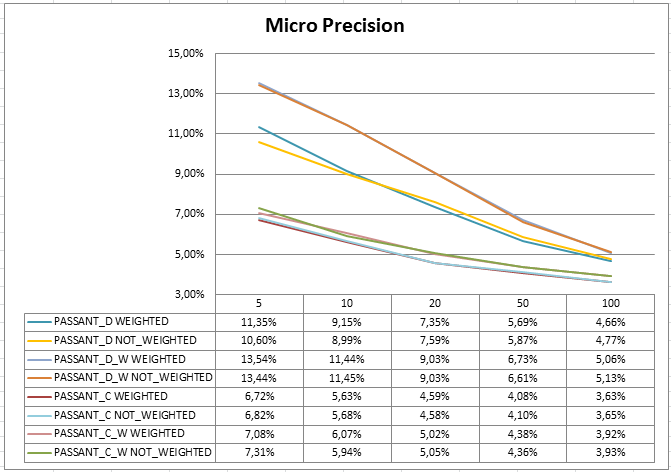
\includegraphics[width=.9\textwidth]{./images/graphs/micro_prec_Own}
	\caption{\emph{Config A - Micro precision}}
\end{figure}

\begin{figure}[H]
	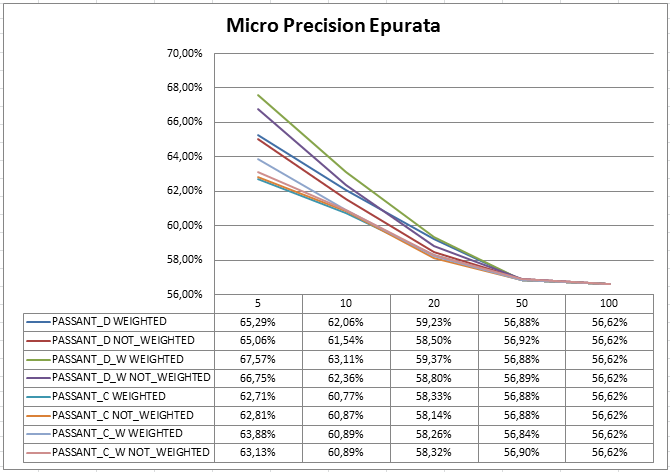
\includegraphics[width=.9\textwidth]{./images/graphs/micro_precT_Own}
	\caption{\emph{Config A - Micro precision epurata}}
\end{figure}

\subsection{Configurazione B}
Testando altri possibili valori da attribuire alle singole proprietà, si sono ottenuti questi risultati:
\begin{table}[H]
	\small
	\centering
	\begin{tabular}{l c}
		\textit{Properties} & \textit{Value} \\\hline
		editing & 0.2 \\
		music & 0.1 \\
		cinematography & 0.1 \\
		director & 0.7 \\
		distributor & 0.1 \\
		producer & 0.1 \\
		starring & 0.6 \\
		studio & 0.1 \\
		writer & 0.3 \\
		subject & 0.8 \\
	\end{tabular}
	\caption{\emph{Configurazione B}}
\end{table}

		% Table generated by 'ConfMusto'
\begin{table}[H]
	\centering
	\resizebox{.9\textwidth}{!}{%
		\begin{tabular}{ c l r c c c c }
			\toprule
			{\bf $K$} & {\bf $DISTANCE$} & {\bf $PROFILE$} & {\bf $\mu\;\pi$} & {\bf $\mu\;\pi\;$Ts} & {\bf $\mu\;MRR$} & {\bf $\mu\;MRR\;$Ts} \\
			\midrule
			
			5 & PASSANT\_D\_W & NOT\_WEIGHTED &    12,10\% &    65,06\% &     7,34\% &    63,05\% \\
			
			5 & PASSANT\_D\_W &   WEIGHTED &    12,01\% &    66,49\% &     7,41\% &    64,17\% \\
			
			5 &  PASSANT\_D &   WEIGHTED &    11,35\% &    65,29\% &     6,65\% &    63,67\% \\
			
			5 &  PASSANT\_D & NOT\_WEIGHTED &    10,60\% &    65,06\% &     6,74\% &    63,03\% \\
			
			10 & PASSANT\_D\_W & NOT\_WEIGHTED &     9,98\% &    61,87\% &     7,34\% &    63,05\% \\
			
			10 & PASSANT\_D\_W &   WEIGHTED &     9,58\% &    62,62\% &     7,41\% &    64,17\% \\
			
			10 &  PASSANT\_D &   WEIGHTED &     9,15\% &    62,06\% &     6,65\% &    63,67\% \\
			
			10 &  PASSANT\_D & NOT\_WEIGHTED &     8,99\% &    61,54\% &     6,74\% &    63,03\% \\
			
			20 & PASSANT\_D\_W & NOT\_WEIGHTED &     8,15\% &    58,66\% &     7,34\% &    63,05\% \\
			
			20 & PASSANT\_D\_W &   WEIGHTED &     7,99\% &    59,36\% &     7,41\% &    64,17\% \\
			
			20 &  PASSANT\_D & NOT\_WEIGHTED &     7,59\% &    58,50\% &     6,74\% &    63,03\% \\
			
			20 &  PASSANT\_D &   WEIGHTED &     7,35\% &    59,23\% &     6,65\% &    63,67\% \\
			
			5 &  PASSANT\_C & NOT\_WEIGHTED &     6,82\% &    62,81\% &     4,69\% &    61,92\% \\
			
			5 &  PASSANT\_C &   WEIGHTED &     6,72\% &    62,71\% &     4,70\% &    62,42\% \\
			
			5 & PASSANT\_C\_W & NOT\_WEIGHTED &     6,49\% &    62,58\% &     4,67\% &    62,08\% \\
			
			5 & PASSANT\_C\_W &   WEIGHTED &     6,17\% &    63,03\% &     4,57\% &    62,24\% \\
			
			50 & PASSANT\_D\_W &   WEIGHTED &     6,14\% &    56,88\% &     7,41\% &    64,17\% \\
			
			50 & PASSANT\_D\_W & NOT\_WEIGHTED &     6,04\% &    56,88\% &     7,34\% &    63,05\% \\
			
			50 &  PASSANT\_D & NOT\_WEIGHTED &     5,87\% &    56,92\% &     6,74\% &    63,03\% \\
			
			50 &  PASSANT\_D &   WEIGHTED &     5,69\% &    56,88\% &     6,65\% &    63,67\% \\
			
			10 &  PASSANT\_C & NOT\_WEIGHTED &     5,68\% &    60,87\% &     4,69\% &    61,92\% \\
			
			10 &  PASSANT\_C &   WEIGHTED &     5,63\% &    60,77\% &     4,70\% &    62,42\% \\
			
			10 & PASSANT\_C\_W & NOT\_WEIGHTED &     5,50\% &    60,73\% &     4,67\% &    62,08\% \\
			
			10 & PASSANT\_C\_W &   WEIGHTED &     5,32\% &    60,38\% &     4,57\% &    62,24\% \\
			
			100 & PASSANT\_D\_W & NOT\_WEIGHTED &     4,96\% &    56,62\% &     7,34\% &    63,05\% \\
			
			100 & PASSANT\_D\_W &   WEIGHTED &     4,85\% &    56,62\% &     7,41\% &    64,17\% \\
			
			100 &  PASSANT\_D & NOT\_WEIGHTED &     4,77\% &    56,62\% &     6,74\% &    63,03\% \\
			
			20 & PASSANT\_C\_W & NOT\_WEIGHTED &     4,76\% &    58,03\% &     4,67\% &    62,08\% \\
			
			100 &  PASSANT\_D &   WEIGHTED &     4,66\% &    56,62\% &     6,65\% &    63,67\% \\
			
			20 & PASSANT\_C\_W &   WEIGHTED &     4,65\% &    58,23\% &     4,57\% &    62,24\% \\
			
			20 &  PASSANT\_C &   WEIGHTED &     4,59\% &    58,33\% &     4,70\% &    62,42\% \\
			
			20 &  PASSANT\_C & NOT\_WEIGHTED &     4,58\% &    58,14\% &     4,69\% &    61,92\% \\
			
			50 & PASSANT\_C\_W & NOT\_WEIGHTED &     4,19\% &    56,89\% &     4,67\% &    62,08\% \\
			
			50 & PASSANT\_C\_W &   WEIGHTED &     4,18\% &    56,88\% &     4,57\% &    62,24\% \\
			
			50 &  PASSANT\_C & NOT\_WEIGHTED &     4,10\% &    56,88\% &     4,69\% &    61,92\% \\
			
			50 &  PASSANT\_C &   WEIGHTED &     4,08\% &    56,88\% &     4,70\% &    62,42\% \\
			
			100 & PASSANT\_C\_W & NOT\_WEIGHTED &     3,80\% &    56,62\% &     4,67\% &    62,08\% \\
			
			100 & PASSANT\_C\_W &   WEIGHTED &     3,78\% &    56,62\% &     4,57\% &    62,24\% \\
			
			100 &  PASSANT\_C & NOT\_WEIGHTED &     3,65\% &    56,62\% &     4,69\% &    61,92\% \\
			
			100 &  PASSANT\_C &   WEIGHTED &     3,63\% &    56,62\% &     4,70\% &    62,42\% \\
			\bottomrule
		\end{tabular}  
	}
	\caption{\emph{Risultati configurazione B}}
\end{table}

\begin{table}[H]
	\centering
	\resizebox{.9\textwidth}{!}{%
		\begin{tabular}{ c l r c c c c }
			\toprule
			{\bf $K$} & {\bf $DISTANCE$} & {\bf $PROFILE$} & {\bf $M\;\pi$} & {\bf $M\;\pi\;$Ts} & {\bf $M\;MRR$} & {\bf $M\;MRR\;$Ts} \\
			\midrule
			
			5 & PASSANT\_D\_W & NOT\_WEIGHTED &    12,10\% &    65,06\% &     7,36\% &    63,57\% \\
			
			5 & PASSANT\_D\_W &   WEIGHTED &    12,01\% &    66,49\% &     7,44\% &    64,57\% \\
			
			5 &  PASSANT\_D &   WEIGHTED &    11,35\% &    65,29\% &     6,68\% &    64,15\% \\
			
			5 &  PASSANT\_D & NOT\_WEIGHTED &    10,60\% &    65,06\% &     6,76\% &    63,58\% \\
			
			10 & PASSANT\_D\_W & NOT\_WEIGHTED &     9,98\% &    62,11\% &     7,36\% &    63,57\% \\
			
			10 & PASSANT\_D\_W &   WEIGHTED &     9,58\% &    62,81\% &     7,44\% &    64,57\% \\
			
			10 &  PASSANT\_D &   WEIGHTED &     9,15\% &    62,29\% &     6,68\% &    64,15\% \\
			
			10 &  PASSANT\_D & NOT\_WEIGHTED &     8,99\% &    61,80\% &     6,76\% &    63,58\% \\
			
			20 & PASSANT\_D\_W & NOT\_WEIGHTED &     8,15\% &    59,79\% &     7,36\% &    63,57\% \\
			
			20 & PASSANT\_D\_W &   WEIGHTED &     7,99\% &    60,30\% &     7,44\% &    64,57\% \\
			
			20 &  PASSANT\_D & NOT\_WEIGHTED &     7,59\% &    59,68\% &     6,76\% &    63,58\% \\
			
			20 &  PASSANT\_D &   WEIGHTED &     7,35\% &    60,21\% &     6,68\% &    64,15\% \\
			
			5 &  PASSANT\_C & NOT\_WEIGHTED &     6,82\% &    62,81\% &     4,71\% &    62,63\% \\
			
			5 &  PASSANT\_C &   WEIGHTED &     6,72\% &    62,71\% &     4,73\% &    63,06\% \\
			
			5 & PASSANT\_C\_W & NOT\_WEIGHTED &     6,49\% &    62,58\% &     4,68\% &    62,79\% \\
			
			5 & PASSANT\_C\_W &   WEIGHTED &     6,17\% &    63,03\% &     4,60\% &    62,91\% \\
			
			50 & PASSANT\_D\_W &   WEIGHTED &     6,14\% &    59,11\% &     7,44\% &    64,57\% \\
			
			50 & PASSANT\_D\_W & NOT\_WEIGHTED &     6,04\% &    59,11\% &     7,36\% &    63,57\% \\
			
			50 &  PASSANT\_D & NOT\_WEIGHTED &     5,87\% &    59,12\% &     6,76\% &    63,58\% \\
			
			50 &  PASSANT\_D &   WEIGHTED &     5,69\% &    59,11\% &     6,68\% &    64,15\% \\
			
			10 &  PASSANT\_C & NOT\_WEIGHTED &     5,68\% &    61,18\% &     4,71\% &    62,63\% \\
			
			10 &  PASSANT\_C &   WEIGHTED &     5,63\% &    61,08\% &     4,73\% &    63,06\% \\
			
			10 & PASSANT\_C\_W & NOT\_WEIGHTED &     5,50\% &    61,05\% &     4,68\% &    62,79\% \\
			
			10 & PASSANT\_C\_W &   WEIGHTED &     5,32\% &    60,72\% &     4,60\% &    62,91\% \\
			
			100 & PASSANT\_D\_W & NOT\_WEIGHTED &     4,96\% &    59,08\% &     7,36\% &    63,57\% \\
			
			100 & PASSANT\_D\_W &   WEIGHTED &     4,85\% &    59,08\% &     7,44\% &    64,57\% \\
			
			100 &  PASSANT\_D & NOT\_WEIGHTED &     4,77\% &    59,08\% &     6,76\% &    63,58\% \\
			
			20 & PASSANT\_C\_W & NOT\_WEIGHTED &     4,76\% &    59,33\% &     4,68\% &    62,79\% \\
			
			100 &  PASSANT\_D &   WEIGHTED &     4,66\% &    59,08\% &     6,68\% &    64,15\% \\
			
			20 & PASSANT\_C\_W &   WEIGHTED &     4,65\% &    59,47\% &     4,60\% &    62,91\% \\
			
			20 &  PASSANT\_C &   WEIGHTED &     4,59\% &    59,55\% &     4,73\% &    63,06\% \\
			
			20 &  PASSANT\_C & NOT\_WEIGHTED &     4,58\% &    59,41\% &     4,71\% &    62,63\% \\
			
			50 & PASSANT\_C\_W & NOT\_WEIGHTED &     4,19\% &    59,11\% &     4,68\% &    62,79\% \\
			
			50 & PASSANT\_C\_W &   WEIGHTED &     4,18\% &    59,11\% &     4,60\% &    62,91\% \\
			
			50 &  PASSANT\_C & NOT\_WEIGHTED &     4,10\% &    59,11\% &     4,71\% &    62,63\% \\
			
			50 &  PASSANT\_C &   WEIGHTED &     4,08\% &    59,11\% &     4,73\% &    63,06\% \\
			
			100 & PASSANT\_C\_W & NOT\_WEIGHTED &     3,80\% &    59,08\% &     4,68\% &    62,79\% \\
			
			100 & PASSANT\_C\_W &   WEIGHTED &     3,78\% &    59,08\% &     4,60\% &    62,91\% \\
			
			100 &  PASSANT\_C & NOT\_WEIGHTED &     3,65\% &    59,08\% &     4,71\% &    62,63\% \\
			
			100 &  PASSANT\_C &   WEIGHTED &     3,63\% &    59,08\% &     4,73\% &    63,06\% \\
			\bottomrule
		\end{tabular}  
}
	\caption{\emph{Risultati configurazione B}}
\end{table}

Analizzando anche in questo caso i valori ottenuti nelle due metriche prese in considerazione anche nella configurazione precedente, otteniamo i seguenti grafici:
\begin{figure}[H]
	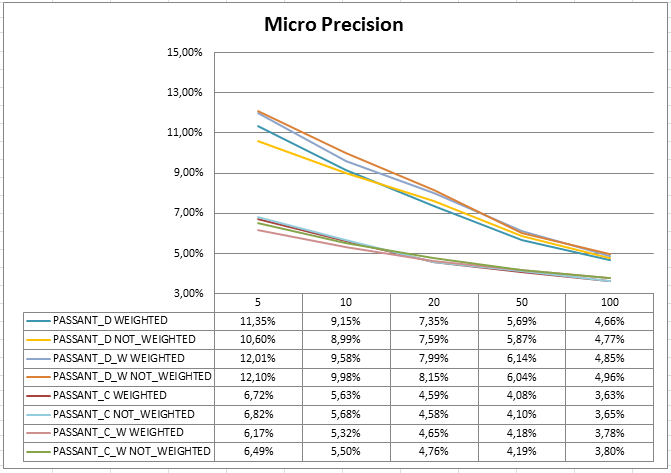
\includegraphics[width=.9\textwidth]{./images/graphs/micro_prec_Musto}
	\caption{\emph{Config B - Micro precision}}
\end{figure}

\begin{figure}[H]
	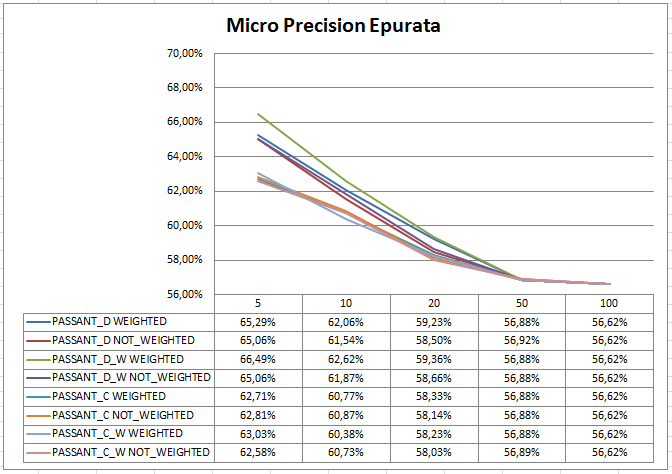
\includegraphics[width=.9\textwidth]{./images/graphs/micro_precT_Musto}
	\caption{\emph{Config B - Micro precision epurata}}
\end{figure}
Cosi come accadeva in precedenza, tipologia che permette di ottenere le prestazioni migliori è sempre a distanza diretta e pesata di Passant in entrambe le varianti di profilazione.

\subsection{Configurazione C}
Di seguito il settaggio della terza configurazione presa in esame con i relativi risultati della raccomandazione: 
\begin{table}[H]
	\small
	\centering
	\begin{tabular}{l l}
		\textit{Properties} & \textit{Value} \\\hline
		editing & 0 \\
		music & 0.31 \\
		cinematography & 0\\
		director & 0.83\\
		distributor & 0\\
		producer & 0 \\
		starring & 0.50\\
		studio & 0\\
		writer & 0\\
		subject & 0.23\\
	\end{tabular}
	\caption{\emph{Configurazione C}}
\end{table}

% Table generated by 'MaxRaggiunto'
\begin{table}[H]
	\centering
	\resizebox{.9\textwidth}{!}{%
\begin{tabular}{ c l r c c c c }
	\toprule
	{\bf $K$} & {\bf $DISTANCE$} & {\bf $PROFILE$} & {\bf $\mu\;\pi$} & {\bf $\mu\;\pi\;$Ts} & {\bf $\mu\;MRR$} & {\bf $\mu\;MRR\;$Ts} \\
	\midrule
	5 & PASSANT\_D\_W &   WEIGHTED &    14,55\% &    68,97\% &     8,89\% &    65,97\% \\
	
	5 & PASSANT\_D\_W & NOT\_WEIGHTED &    13,93\% &    67,73\% &     8,60\% &    64,67\% \\
	
	10 & PASSANT\_D\_W &   WEIGHTED &    12,51\% &    63,51\% &     8,89\% &    65,97\% \\
	
	10 & PASSANT\_D\_W & NOT\_WEIGHTED &    12,09\% &    62,81\% &     8,60\% &    64,67\% \\
	
	5 &  PASSANT\_D &   WEIGHTED &    11,35\% &    65,29\% &     6,65\% &    63,67\% \\
	
	5 &  PASSANT\_D & NOT\_WEIGHTED &    10,60\% &    65,06\% &     6,74\% &    63,03\% \\
	
	5 & PASSANT\_C\_W &   WEIGHTED &    10,15\% &    65,12\% &     6,48\% &    63,22\% \\
	
	20 & PASSANT\_D\_W & NOT\_WEIGHTED &    10,06\% &    59,06\% &     8,60\% &    64,67\% \\
	
	20 & PASSANT\_D\_W &   WEIGHTED &    10,02\% &    59,72\% &     8,89\% &    65,97\% \\
	
	5 & PASSANT\_C\_W & NOT\_WEIGHTED &     9,85\% &    64,50\% &     6,13\% &    62,69\% \\
	
	10 &  PASSANT\_D &   WEIGHTED &     9,15\% &    62,06\% &     6,65\% &    63,67\% \\
	
	10 &  PASSANT\_D & NOT\_WEIGHTED &     8,99\% &    61,54\% &     6,74\% &    63,03\% \\
	
	10 & PASSANT\_C\_W &   WEIGHTED &     7,65\% &    61,80\% &     6,48\% &    63,22\% \\
	
	20 &  PASSANT\_D & NOT\_WEIGHTED &     7,59\% &    58,50\% &     6,74\% &    63,03\% \\
	
	20 &  PASSANT\_D &   WEIGHTED &     7,35\% &    59,23\% &     6,65\% &    63,67\% \\
	
	10 & PASSANT\_C\_W & NOT\_WEIGHTED &     7,29\% &    61,40\% &     6,13\% &    62,69\% \\
	
	50 & PASSANT\_D\_W &   WEIGHTED &     7,20\% &    56,94\% &     8,89\% &    65,97\% \\
	
	50 & PASSANT\_D\_W & NOT\_WEIGHTED &     7,05\% &    56,92\% &     8,60\% &    64,67\% \\
	
	5 &  PASSANT\_C & NOT\_WEIGHTED &     6,82\% &    62,81\% &     4,69\% &    61,92\% \\
	
	5 &  PASSANT\_C &   WEIGHTED &     6,72\% &    62,71\% &     4,70\% &    62,42\% \\
	
	20 & PASSANT\_C\_W &   WEIGHTED &     5,98\% &    58,66\% &     6,48\% &    63,22\% \\
	
	50 &  PASSANT\_D & NOT\_WEIGHTED &     5,87\% &    56,92\% &     6,74\% &    63,03\% \\
	
	50 &  PASSANT\_D &   WEIGHTED &     5,69\% &    56,88\% &     6,65\% &    63,67\% \\
	
	10 &  PASSANT\_C & NOT\_WEIGHTED &     5,68\% &    60,87\% &     4,69\% &    61,92\% \\
	
	20 & PASSANT\_C\_W & NOT\_WEIGHTED &     5,65\% &    58,48\% &     6,13\% &    62,69\% \\
	
	10 &  PASSANT\_C &   WEIGHTED &     5,63\% &    60,77\% &     4,70\% &    62,42\% \\
	
	100 & PASSANT\_D\_W &   WEIGHTED &     5,31\% &    56,62\% &     8,89\% &    65,97\% \\
	
	100 & PASSANT\_D\_W & NOT\_WEIGHTED &     5,30\% &    56,62\% &     8,60\% &    64,67\% \\
	
	50 & PASSANT\_C\_W &   WEIGHTED &     5,09\% &    56,87\% &     6,48\% &    63,22\% \\
	
	50 & PASSANT\_C\_W & NOT\_WEIGHTED &     4,92\% &    56,89\% &     6,13\% &    62,69\% \\
	
	100 &  PASSANT\_D & NOT\_WEIGHTED &     4,77\% &    56,62\% &     6,74\% &    63,03\% \\
	
	100 &  PASSANT\_D &   WEIGHTED &     4,66\% &    56,62\% &     6,65\% &    63,67\% \\
	
	20 &  PASSANT\_C &   WEIGHTED &     4,59\% &    58,33\% &     4,70\% &    62,42\% \\
	
	20 &  PASSANT\_C & NOT\_WEIGHTED &     4,58\% &    58,14\% &     4,69\% &    61,92\% \\
	
	100 & PASSANT\_C\_W &   WEIGHTED &     4,25\% &    56,62\% &     6,48\% &    63,22\% \\
	
	100 & PASSANT\_C\_W & NOT\_WEIGHTED &     4,15\% &    56,62\% &     6,13\% &    62,69\% \\
	
	50 &  PASSANT\_C & NOT\_WEIGHTED &     4,10\% &    56,88\% &     4,69\% &    61,92\% \\
	
	50 &  PASSANT\_C &   WEIGHTED &     4,08\% &    56,88\% &     4,70\% &    62,42\% \\
	
	100 &  PASSANT\_C & NOT\_WEIGHTED &     3,65\% &    56,62\% &     4,69\% &    61,92\% \\
	
	100 &  PASSANT\_C &   WEIGHTED &     3,63\% &    56,62\% &     4,70\% &    62,42\% \\
	\bottomrule
	\end{tabular}  	
}
	\caption{\emph{Risultati configurazione C}}
\end{table}

\begin{table}[H]
	\centering
	\resizebox{.9\textwidth}{!}{%
		\begin{tabular}{ c l r c c c c }
			\toprule
			{\bf $K$} & {\bf $DISTANCE$} & {\bf $PROFILE$} & {\bf $M\;\pi$} & {\bf $M\;\pi\;$Ts} & {\bf $M\;MRR$} & {\bf $M\;MRR\;$Ts} \\
			\midrule
			5 & PASSANT\_D\_W &   WEIGHTED &    14,55\% &    68,97\% &     8,94\% &    66,24\% \\
			
			5 & PASSANT\_D\_W & NOT\_WEIGHTED &    13,93\% &    67,73\% &     8,63\% &    65,05\% \\
			
			10 & PASSANT\_D\_W &   WEIGHTED &    12,51\% &    63,64\% &     8,94\% &    66,24\% \\
			
			10 & PASSANT\_D\_W & NOT\_WEIGHTED &    12,09\% &    62,99\% &     8,63\% &    65,05\% \\
			
			5 &  PASSANT\_D &   WEIGHTED &    11,35\% &    65,29\% &     6,68\% &    64,15\% \\
			
			5 &  PASSANT\_D & NOT\_WEIGHTED &    10,60\% &    65,06\% &     6,76\% &    63,58\% \\
			
			5 & PASSANT\_C\_W &   WEIGHTED &    10,15\% &    65,12\% &     6,51\% &    63,75\% \\
			
			20 & PASSANT\_D\_W & NOT\_WEIGHTED &    10,06\% &    60,08\% &     8,63\% &    65,05\% \\
			
			20 & PASSANT\_D\_W &   WEIGHTED &    10,02\% &    60,57\% &     8,94\% &    66,24\% \\
			
			5 & PASSANT\_C\_W & NOT\_WEIGHTED &     9,85\% &    64,50\% &     6,15\% &    63,27\% \\
			
			10 &  PASSANT\_D &   WEIGHTED &     9,15\% &    62,29\% &     6,68\% &    64,15\% \\
			
			10 &  PASSANT\_D & NOT\_WEIGHTED &     8,99\% &    61,80\% &     6,76\% &    63,58\% \\
			
			10 & PASSANT\_C\_W &   WEIGHTED &     7,65\% &    62,05\% &     6,51\% &    63,75\% \\
			
			20 &  PASSANT\_D & NOT\_WEIGHTED &     7,59\% &    59,68\% &     6,76\% &    63,58\% \\
			
			20 &  PASSANT\_D &   WEIGHTED &     7,35\% &    60,21\% &     6,68\% &    64,15\% \\
			
			10 & PASSANT\_C\_W & NOT\_WEIGHTED &     7,29\% &    61,67\% &     6,15\% &    63,27\% \\
			
			50 & PASSANT\_D\_W &   WEIGHTED &     7,20\% &    59,13\% &     8,94\% &    66,24\% \\
			
			50 & PASSANT\_D\_W & NOT\_WEIGHTED &     7,05\% &    59,12\% &     8,63\% &    65,05\% \\
			
			5 &  PASSANT\_C & NOT\_WEIGHTED &     6,82\% &    62,81\% &     4,71\% &    62,63\% \\
			
			5 &  PASSANT\_C &   WEIGHTED &     6,72\% &    62,71\% &     4,73\% &    63,06\% \\
			
			20 & PASSANT\_C\_W &   WEIGHTED &     5,98\% &    59,79\% &     6,51\% &    63,75\% \\
			
			50 &  PASSANT\_D & NOT\_WEIGHTED &     5,87\% &    59,12\% &     6,76\% &    63,58\% \\
			
			50 &  PASSANT\_D &   WEIGHTED &     5,69\% &    59,11\% &     6,68\% &    64,15\% \\
			
			10 &  PASSANT\_C & NOT\_WEIGHTED &     5,68\% &    61,18\% &     4,71\% &    62,63\% \\
			
			20 & PASSANT\_C\_W & NOT\_WEIGHTED &     5,65\% &    59,66\% &     6,15\% &    63,27\% \\
			
			10 &  PASSANT\_C &   WEIGHTED &     5,63\% &    61,08\% &     4,73\% &    63,06\% \\
			
			100 & PASSANT\_D\_W &   WEIGHTED &     5,31\% &    59,08\% &     8,94\% &    66,24\% \\
			
			100 & PASSANT\_D\_W & NOT\_WEIGHTED &     5,30\% &    59,08\% &     8,63\% &    65,05\% \\
			
			50 & PASSANT\_C\_W &   WEIGHTED &     5,09\% &    59,10\% &     6,51\% &    63,75\% \\
			
			50 & PASSANT\_C\_W & NOT\_WEIGHTED &     4,92\% &    59,11\% &     6,15\% &    63,27\% \\
			
			100 &  PASSANT\_D & NOT\_WEIGHTED &     4,77\% &    59,08\% &     6,76\% &    63,58\% \\
			
			100 &  PASSANT\_D &   WEIGHTED &     4,66\% &    59,08\% &     6,68\% &    64,15\% \\
			
			20 &  PASSANT\_C &   WEIGHTED &     4,59\% &    59,55\% &     4,73\% &    63,06\% \\
			
			20 &  PASSANT\_C & NOT\_WEIGHTED &     4,58\% &    59,41\% &     4,71\% &    62,63\% \\
			
			100 & PASSANT\_C\_W &   WEIGHTED &     4,25\% &    59,08\% &     6,51\% &    63,75\% \\
			
			100 & PASSANT\_C\_W & NOT\_WEIGHTED &     4,15\% &    59,08\% &     6,15\% &    63,27\% \\
			
			50 &  PASSANT\_C & NOT\_WEIGHTED &     4,10\% &    59,11\% &     4,71\% &    62,63\% \\
			
			50 &  PASSANT\_C &   WEIGHTED &     4,08\% &    59,11\% &     4,73\% &    63,06\% \\
			
			100 &  PASSANT\_C & NOT\_WEIGHTED &     3,65\% &    59,08\% &     4,71\% &    62,63\% \\
			
			100 &  PASSANT\_C &   WEIGHTED &     3,63\% &    59,08\% &     4,73\% &    63,06\% \\
			\bottomrule
		\end{tabular}  		 	
	}
	\caption{\emph{Risultati configurazione C}}
\end{table}

Come nei due casi precedenti, verranno analizzati sia la microprecision che la microprecision epurata:
\begin{figure}[H]
	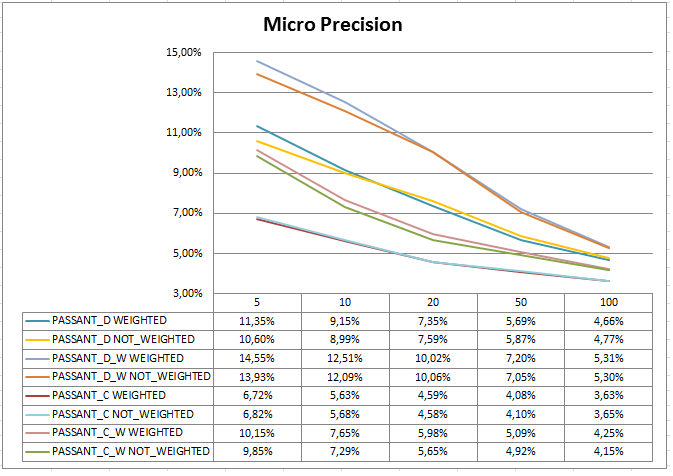
\includegraphics[width=.9\textwidth]{./images/graphs/micro_prec_Best}
	\caption{\emph{Config C - Micro precision}}
\end{figure}

\begin{figure}[H]
	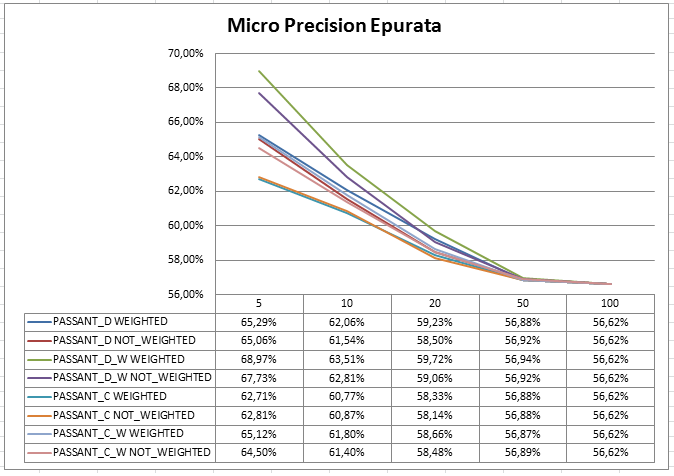
\includegraphics[width=.9\textwidth]{./images/graphs/micro_precT_Best}
	\caption{\emph{Config C - Micro precision epurata}}
\end{figure}

Come si evince da questi grafici, anche in questo caso, i risultati migliori sono quelli espressi sempre dalla distanza diretta e pesata di Passant in entrambe le versioni di profilazione. 

\subsection{Considerazioni}
Mettendo a confronto i risultati migliori ottenuti dalle diverse configurazioni, si evince che la configurazione che ha fatto ottenere i risultati migliori sia in termini di precisione, che in termini di precisione epurata, sia stata l'ultima configurazione presa in esame.

\subsubsection{Microprecision}
In particolar modo, per quanto riguarda la microprecision, ecco un grafico riassuntivo che mette a confronto i risultati migliori ottenuti dalle tre configurazioni:

\begin{figure}
\begin{tikzpicture}
	\begin{axis}[
		/tikz/font={\scriptsize},
		xmin=5,
		xmax=100,
		ymin=4,
		ymax=15,
		ylabel=$Precision (\%)$,
		xlabel= $k$,
		minor grid style={gray!30},
		major grid style={black!50},
		/pgfplots/xtick={5,10,20,50,100},
		/pgfplots/ytick={4,...,15},
		grid=major,
		extra y ticks={4.1,4.2,...,4.9,5.1,5.2,...,5.9,
					6.1,6.2,...,6.9,7.1,7.2,...,7.9,8.1,8.2,...,8.9,
					9.1,9.2,...,9.9,10.1,10.2,...,10.9,11.1,11.2,...,11.9,
					12.1,12.2,...,12.9,13.1,13.2,...,13.9,14.1,14.2,...,14.9},
		mark=none,
		extra y tick style={yticklabels={},grid=minor,tiny,ytick pos=left},
		width=.9\textwidth,
		height=.8\textwidth,
		grid=both, 
		axis background/.style={fill=white}]
		\addplot[color=silver,thick] coordinates {
			(5,13.54)
			(10,11.44)
			(20,9.03)
			(50,6.73)
			(100,5.06)
			
		};
		\addlegendentry{Config A} % conf A = nostra
		
		\addplot[color=bronze,thick] coordinates {
			(5,12.10)
			(10,9.98)
			(20,8.15)
			(50,6.04)
			(100,4.85)
		};
		\addlegendentry{Config B} % conf B = musto
		
		\addplot[color=gold,thick] coordinates {
			(5,14.55)
			(10,12.51)
			(20,10.02)
			(50,7.20)
			(100,5.31)
		};
		\addlegendentry{Config C} % conf C = max raggiunto
		
		\addplot[color=black,thick] coordinates {
			(5,11.35)
			(10,9.15)
			(20,7.35)
			(50,5.69)
			(100,4.66)
		};
		\addlegendentry{\color{red}Baseline}
	\end{axis}
\end{tikzpicture}
\caption{\emph{Confronto delle migliori precision}}
\end{figure}
Come si può constatare, prendendo in considerazione le pesature non omogenee tra gli archi, si è riusciti ad ottenere un miglioramento percentuale della precisione nel sistema di raccomandazione pari a :

\begin{itemize}
	\item +3.2 \% per $k = 5 $
	\item +3.36 \% per $k = 10 $
	\item +2.67 \% per $k = 20 $
	\item +1.51 \% per $k = 50 $
	\item +0.65 \% per $k = 100 $				
\end{itemize} 

\subsubsection{Microprecision Epurata}
Prendendo in considerazione invece le microprecision epurate, otteniamo i seguenti risultati:
\begin{figure}
	\begin{tikzpicture}
	\begin{axis}[
	/tikz/font={\scriptsize},
	xmin=5,     
	xmax=100,    
	ymin=56,
	ymax=69,     
	ylabel=$Precision (\%)$,
	xlabel= $k$,
	minor grid style={gray!20},
	major grid style={black!40},
	/pgfplots/xtick={5,10,20,50,100},
	/pgfplots/ytick={56,...,69},
	grid=major,
	extra y ticks={56.1,56.2,...,56.9,57.1,57.2,...,57.9,58.1,58.2,...,58.9,
					59.1,59.2,...,59.9,60.1,60.2,...,60.9,61.1,61.2,...,61.9,
					62.1,62.2,...,62.9,63.1,63.2,...,63.9,64.1,64.2,...,64.9,
					65.1,65.2,...,65.9,66.1,66.2,...,66.9,67.1,67.2,...,67.9},
	mark=none,
	extra y tick style={yticklabels={},grid=minor,tiny,ytick pos=left},
	legend style={
		%font=\tiny,
		%pos=outer north east,
		%line width=.1pt,
		%mark size=.6pt
	},
	width=.9\textwidth,
	height=.8\textwidth,
	grid=both, 
	axis background/.style={fill=white}]
	\addplot[color=silver,thick] coordinates {
		(5,67.57)
		(10,63.11)
		(20,59.37)
		(50,56.88)
		(100,56.62)
		
	};
	\addlegendentry{Config A} % conf A = nostra
	
	\addplot[color=bronze,thick] coordinates {
		(5,66.49)
		(10,62.62)
		(20,59.36)
		(50,56.88)
		(100,56.62)
	};
	\addlegendentry{Config B} % conf B = musto
	
	\addplot[color=gold,thick] coordinates {
		(5,68.97)
		(10,63.51)
		(20,59.72)
		(50,56.94)
		(100,56.62)
	};
	\addlegendentry{Config C} % conf C = max raggiunto
	
	\addplot[color=black,thick] coordinates {
		(5,65.29)
		(10,62.06)
		(20,59.23)
		(50,56.88)
		(100,56.62)
	};
	\addlegendentry{\color{red}Baseline}
	\end{axis}
	\end{tikzpicture}
	\caption{\emph{Confronto delle migliori precision epurate}}
\end{figure}

Anche in questo caso si può constatare che, prendendo in considerazione le pesature non omogenee tra gli archi, si è riusciti ad ottenere un miglioramento percentuale della precisione nel sistema di raccomandazione pari a :

\begin{itemize}
	\item +3.68 \% per $k = 5 $
	\item +1.45 \% per $k = 10 $
	\item +0.49 \% per $k = 20 $
	\item +0.06 \% per $k = 50 $
	\item 0 \% per $k = 100 $ ~\footnote{Non si è riuscito ad ottenere nessun miglioramento a causa della quantità di film profilati dagli utenti (< 100).}				
\end{itemize} 

	
	\bibliographystyle{abbrvnat}
	\bibliography{mybib}

\end{document}
